\chapter{Unión de imágenes}
\label{capitulo5}
\lhead{Capítulo 5. \emph{Unión de imágenes}}


\section{Introducción}
El objetivo final de la creación de un mosaico, es lograr un mapa que represente de la mejor forma la trayectoria recorrida. Esto es, que sea visualmente congruente y que no presente ningún tipo de discontinuidades de modo que todo parezca una misma imagen. De las primeras etapas se manifiestan muchos errores producto de los problemas ya planteados, si bien a lo largo del proceso éstos se intentan reducir lo mas posible, siempre es necesaria la etapa final de fusión para lograr los objetivos propuestos.

En esta sección se describen los algoritmos utilizados para lograr fusionar las imágenes del mosaico. Como ya se especificó, fueron seleccionados aquellos que presentaron resultados importantes en diversos estudios externos, y se implementaron en conjunto para lograr resultados mucho mas robustos. Estos se detallan a continuación en el orden de aplicación sobre el mosaico: linea de corte, ajuste de color y finalmente la fusión ponderada.

Por ultimo, al final del capítulo se muestran los resultados con su respectivo análisis de aplicar cada uno de los algoritmos aquí descritos.
\clearpage


\section{Linea de costura}\label{seccion-corte}

Este es el primer algoritmo aplicado al mosaico luego de todas las correcciones geométricas, ya que el resto de métodos requieren conocer de antemano los límites de cada imagen. 
A diferencia de los anteriores, este tipo de algoritmos es el único que toma en cuenta la información que comparten las imágenes en el área que tienen en común, con lo cual su implementación logra corregir la mayor cantidad de imperfecciones. 


\subsection{Modelo por grafo}

Este es un método derivado de la teoría de grafos, donde la idea es separar un grafo con conexiones simples en dos grafos separados con un mínimo costo de separación. Se define un grafo $\mathcal{G} = \langle \mathcal{N}, \mathcal{E} \rangle$ como un conjunto de nodos $\mathcal{N}$, conectados por enlaces $\mathcal{E}$. Cada enlace conecta dos nodos y tiene asociado un costo o peso $\mathcal{W}(p, q) \,\, p,q \in \mathcal{N}$ --- cuando se habla de conexión simple, se refiere a que el costo en los enlaces está asociado para ambas direcciones $\mathcal{W}(p, q) = \mathcal{W}(p, q)$ ---. Se dice que dos grafos están separados si no se tiene ningún enlace que conecte dos nodos entre los grafos. Definimos $\mathcal{S}$ y $\mathcal{T}$ como los grafos separados que se tienen luego de aplicar el corte en $\mathcal{G}$. El método para determinar el mejor corte, se basa en encontrar el camino entre los enlaces que logra separa un grafo en dos, con el mínimo costo de corte \cite{graph-cut}, donde el costo del corte es la suma de los pesos de todos los enlaces del camino seleccionado.

En el conjunto de nodos presentes en el grafo se cuentan con dos especiales llamados nodos terminales, el inicio ($\mathtt{I}$) y el final ($\mathtt{F}$), donde el resto de píxeles en la imagen corresponden con un nodo no terminal. En aplicaciones de visión por computadora, cuando se desea unir dos imágenes en una región de intersección, lo que se busca es lograr un etiquetado de píxeles que permita distinguir que nodos corresponden a cada imagen en el área de intersección.

Se presenta en la ecuación \ref{funcion-corte} la función de coste que etiqueta los nodos, y minimiza el costo del corte.
\begin{equation}
C(f) = \sum_{_p\in \mathcal{N}}^{} D_p(f_p) + \sum_{_p,_q \in \mathcal{N} - \{\mathtt{I},\mathtt{F}\}}^{} \mathcal{W}_p,_q (f_p, f_q)
\label{funcion-corte}
\end{equation}
Donde $p$ es un nodo que pertenece al conjunto de nodos no terminales $\mathcal{N} - \{\mathtt{I},\mathtt{F}\}$. El término $D_p(f_p)$ es el costo de asignar una etiqueta $f_p$ ($f_p \in \{0,\,1\}$) al nodo $p$ --- en este caso una etiqueta binaria, asociando el píxel a una imagen u otra ---. El término $\mathcal{W}_{p,q} (f_p, f_q)$ es el costo de asociar una etiqueta al nodo $p$ y una distinta al nodo $q$.

Una gran diferencia de intensidades entre píxeles adyacentes representa un fuerte indicador de la existencia de un borde o contorno entre dos objetos, es decir, que el costo de un enlace se puede definir como el inverso de la diferencia entre la intensidad de los píxeles que conecta. Siendo $I(p)$ la intensidad de un píxel $p$, se defina el coso de cada enlace como:
\begin{equation}
\mathcal{W}_p,_q = 255 - |I(p) - I (q)|
\label{costo-corte}
\end{equation}
Si bien se consideran los parámetros necesarios con esa función, se obtienen resultados mucho mas robustos usando una función exponencial \cite{graph-opencv}:
\begin{equation}
\mathcal{W}_p,_q = e^{\left(\frac{255-|I(p) - I (q)|}{2 \sigma}  \right) }
\label{costo-corte}
\end{equation}
Donde $\sigma$ es la desviación estándar de la imagen, y siendo válido para los casos en los que $f_p \neq f_q$. Esto indica que dos nodos continuos pertenecen a distintos grafos ($\mathcal{S,T}$) y a su vez que son separados por la linea de corte.

\begin{figure}[h]
	\centering
	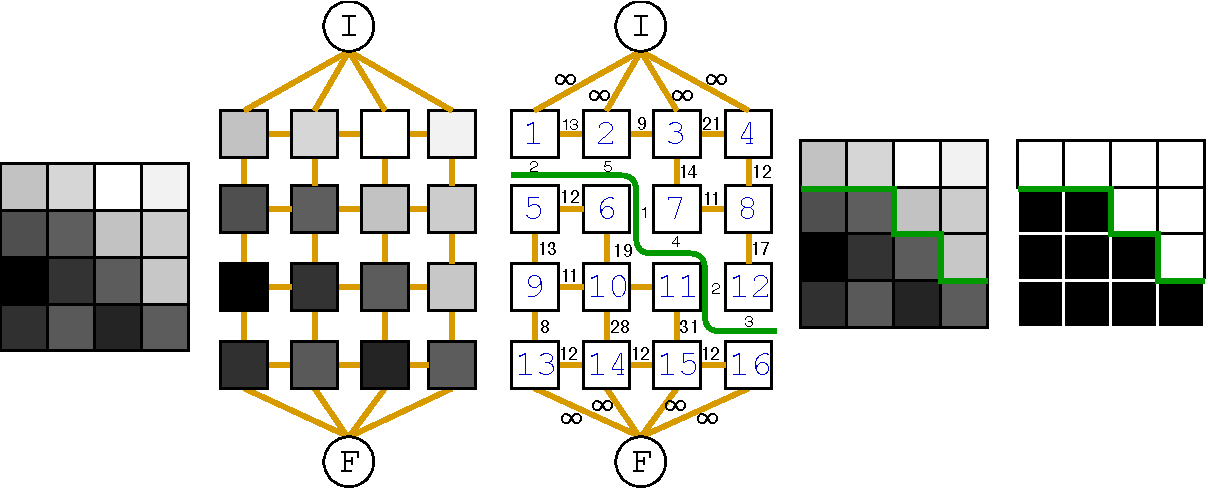
\includegraphics[width=1\linewidth]{grafo-completo.pdf}
	\caption[Corte por grafo]{De izquierda a derecha: imagen original, creación de nodos y enlaces, se asignan los pesos y se halla la linea de corte, finalmente se binariza la imagen según las etiquetas para crear una mascara.}
	\label{imagen:grafo}
\end{figure}

Refiriéndonos a la figura \ref{imagen:grafo}, se observa el proceso de modelar una imagen mediante un grafo con conexiones simples y usando un esquema de 4 vecindad --- 4 vecindad solo considera a los píxeles superior, inferior y laterales como vecinos ---, donde cada cuadro está compuesto por el inverso de la diferencia de intensidades entre dos imágenes, representado en escala de grises. Al final se tiene una imagen compuesta por dos grafos separados, donde $\mathtt{I} \in \mathcal{S}$ y $\mathtt{F} \in \mathcal{T}$ donde a cada nodo del grafo se le asigna un valor binario dependiendo de la etiqueta resultante el algoritmo de minimización del costo de corte.


\section{Corrección de color}\label{seccion-color}
Cuando se tienen imágenes capturadas desde distintos puntos de vista, se suelen tener en la composición final cambios de intensidades, debido a cambios de exposición de luz en la escena. Por ellos es necesario implementar algoritmos que logran reducir la diferencia de intensidades y color entre los bordes de las imágenes. Para esto se implementa un algoritmo de mapeo de color llamado método de \textit{Reinhard} \cite{reinhard} que trabaja en el espacio de color CIELAB, descrito a continuación. 

\subsubsection*{Espacio de color CIELAB}

Conocido en ocasiones con el nombre de l*a*b, es un espacio derivado del \textit{CIE 1931 XYZ}, creado por la comisión internacional de la iluminación CIE (del francés: Comission Internationale de l'Éclairage).

\begin{figure}[h]
	\centering     %%% not \center
	\subfigure[]{\label{fig:lab-a}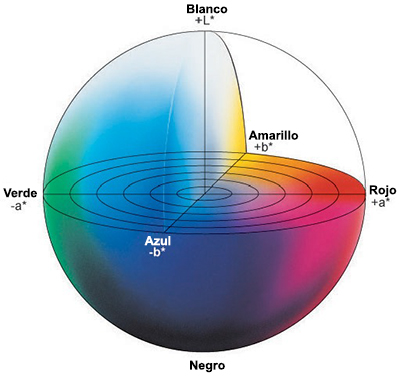
\includegraphics[width=.42\textwidth]{lab1}}
	\subfigure[]{\label{fig:lab-b}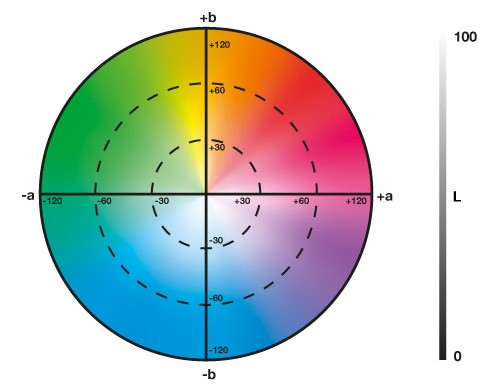
\includegraphics[width=.50\textwidth]{lab2}}
	
	\caption[Espacio de color CIELAB]{Espacio de color CIELAB. En (a) se aprecia el diagrama tridimensional, mientras que en (b) una vista superior del rango de colores con luminancia fija.}
	\label{imagen:lab-color}
\end{figure}

Este es un espacio de color tridimensional descrito por los ejes $a$, que extiende desde verde ($-a$) hasta rojo ($+a$), el eje $b$ que se extiende desde azul ($-b$) hasta amarillo ($+b$), y la luminancia $l$ que varia desde negro ($-l$) hasta blanco ($+l$). Esta representación se puede observar en la figura \ref{imagen:lab-color}.

Debido a que la cantidad de valores para representar los colores en este espacio es menor que en RGB, es mas rápido hacer correcciones de color en LAB, ya que un cambio en la cantidad de valor de una variable produce un cambio con importancia visual. Además de permitir trabajar la iluminación de la imagen por separado de los colores.

\subsection{Método de Reinhard}
El objetivo de esta transformación de color es lograr que la distribución de los puntos en el espacio de color LAB se transfieran entre imágenes. Para esto se utiliza la información de la media y desviación estándar sobre cada canal (L, A y B).

Para un par de imágenes $I$ e $I^*$, donde $I$ es la imagen origen e $I^*$ es la imagen que se quiere corregir, se calcula la media y desviación estándar para cada canal.
\begin{align*}
&{\langle l \rangle} \hspace{0.55cm} {\langle l^* \rangle}  &{ \sigma_l } \hspace{0.5cm} { \sigma^*_l } \\
&{\langle a \rangle} \hspace{0.48cm} {\langle a^* \rangle}  &{ \sigma_a } \hspace{0.5cm} { \sigma^*_a }  \\
&{\langle b \rangle} \hspace{0.5cm} {\langle b^* \rangle}  &{ \sigma_b } \hspace{0.5cm} { \sigma^*_b } 
\end{align*}
Luego se ajusta la distribución de la imagen objetivo restandole la media obtenida en el paso anterior:
\begin{align*}
l^* &= l^* - \langle l^* \rangle \\
a^* &= a^* - \langle a^* \rangle \\
b^* &= b^* - \langle b^* \rangle
\end{align*}
Luego se escalan los valores en función a las desviaciones estándar:
\begin{align*}
l^* &= \frac{\sigma^*_l}{\sigma_l} l^* \\
a^* &= \frac{\sigma^*_a}{\sigma_a} a^* \\
b^* &= \frac{\sigma^*_b}{\sigma_b} b^*
\end{align*}
Finalmente se le suma la media, pero en este caso de la imagen de origen (imagen del color deseado):
\begin{align*}
l^* &= l^* + \langle l \rangle \\
a^* &= a^* + \langle a \rangle \\
b^* &= b^* + \langle b \rangle
\end{align*}
Para lograr un mapeo de color correcto es necesario obtener la información de desviación estándar y media únicamente en el área de intersección entre las imágenes $I\cap I^*$. De esta forma se logra igualar estas regiones de la imagen que deben corresponder a la misma escena.


\section{Fusión de imágenes}\label{seccion-fusion}

Una vez se logre determinar la mejor linea de corte, y aplicar una corrección de color, es posible que aun se cuenten con transiciones entre imágenes con cierto nivel de discontinuidad. En este caso es conveniente aplicar algoritmos que permitan una transición suavizada entre dichos bordes.

Se tienen varias versiones de estos algoritmos que serán explicados a continuación: fusión ponderada simple o bajo un esquema piramidal.

\subsection{Fusión ponderada} \label{feathering}
Este tipo de algoritmos realiza una fusión que consiste en realizar un suma ponderada, en la cual se modifica el peso de los píxeles en función de la distancia con el borde de su imagen. Es decir, se realiza una suma de los valores de las imágenes ($\mathtt{I_1},\, \mathtt{I_2}$) en el área de intersección ($\mathtt{I_1}\cap \mathtt{I_2}$) para cada canal, dándole menor peso a los píxeles que se encuentren mas cercanos del extremo de la imagen. Cabe destacar que esta suma se normaliza para asegurar que no se supere el rango $0-255$ con el cual se representan los valores de la imagen final. La ecuación para la suma ponderada se muestra a continuación:
\begin{displaymath}
	F = (1-\alpha)\cdot \mathtt{I}_1 + \alpha\cdot \mathtt{I}_2
\end{displaymath} 
Donde el parámetro $\alpha$ varia en el rango $0\to 1$, en este caso en función a la distancia, tal y como se ilustra en la figura \ref{imagen:blend-simple}.


\begin{figure}[h]
	\centering
	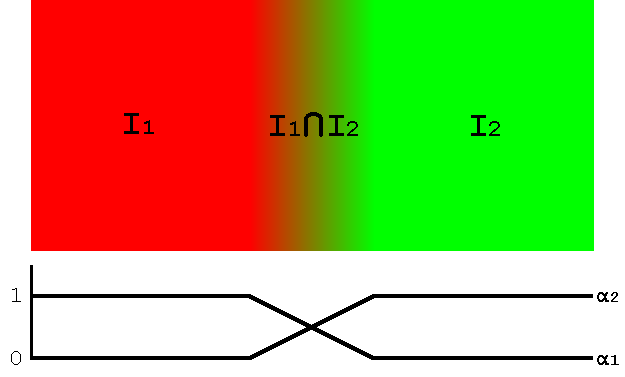
\includegraphics[width=.6\linewidth]{blend1.pdf}
	\caption[Fusión ponderada simple]{Fusión ponderada simple, donde $\alpha_1$ y $\alpha_2$ corresponden con el factor multiplicativo de las imágenes 1 y 2 respectivamente ($\alpha_1 = 1 - \alpha_2$).}
	\label{imagen:blend-simple}
\end{figure}

El algoritmo de fusión ponderada bajo el esquema de transición presenta ciertas desventajas, entre estas el efecto fantasma, en el que se observan duplicados de los objetos en la escena pero con cierto grado de desvanecimiento. Si bien no será implementado, el estudio de su funcionamiento es necesario para comprender el algoritmo de fusión que trabaja bajo un esquema piramidal.

\subsection{Fusión ponderada piramidal}

El método planteado anteriormente propone una transición suavizada para imágenes que tengan una región en común. Si bien es una primera aproximación al problema aquí planteado, los algoritmos que se pretenden utilizar en etapas previas (linea de corte) eliminan ésta área de intersección, quedando don imágenes con solo un borde en común. 

Esta técnica es llamada fusión piramidal o fusión multibanda, y su proceso consiste en fusionar las imágenes para distintos niveles de escala. Refiriéndonos a la figura \ref{imagen:piramidal1}, se crea para una misma imagen distintos niveles de escala ($G_i$), donde cada nivel corresponde con una reducción a un cuarto del área del nivel anterior. La cantidad de niveles en la pirámide corresponde con la cantidad de bandas que se quieren fusionar. Es importante mencionar que el proceso de compresión y posterior expansión de una imagen, se aproxima al proceso de aplicar un filtro gaussiano, con lo cual a cada nivel creado $G_i$ recibe el nombre de gaussiana, resultando lo que se denomina una pirámide de gaussianas, tal y como se ilustra en la figura \ref{imagen:piramidal1} con 5 niveles.

\begin{figure}[h]
	\centering
	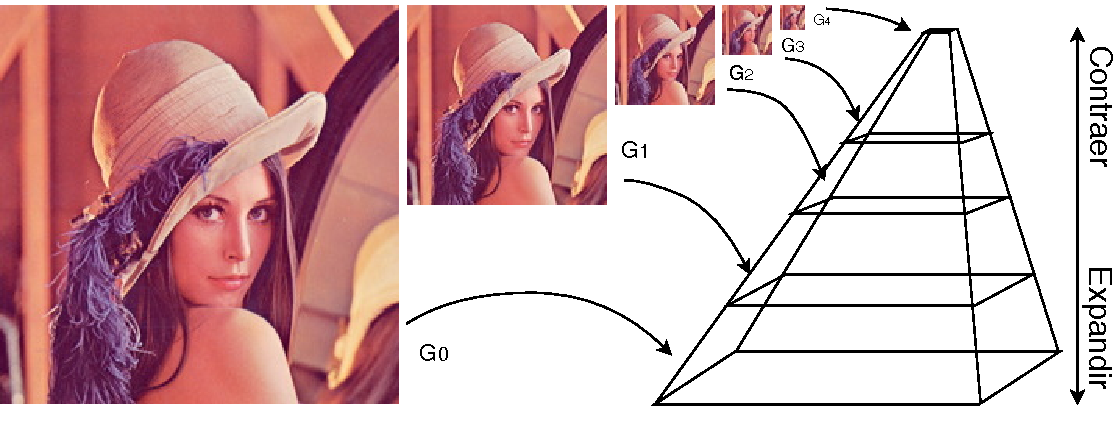
\includegraphics[width=.8\linewidth]{piramidal1.pdf}
	\caption[Construcción de pirámide de gaussianas]{Construcción de pirámide de gaussianas}
	\label{imagen:piramidal1}
\end{figure}



\begin{figure}[h]
	\centering
	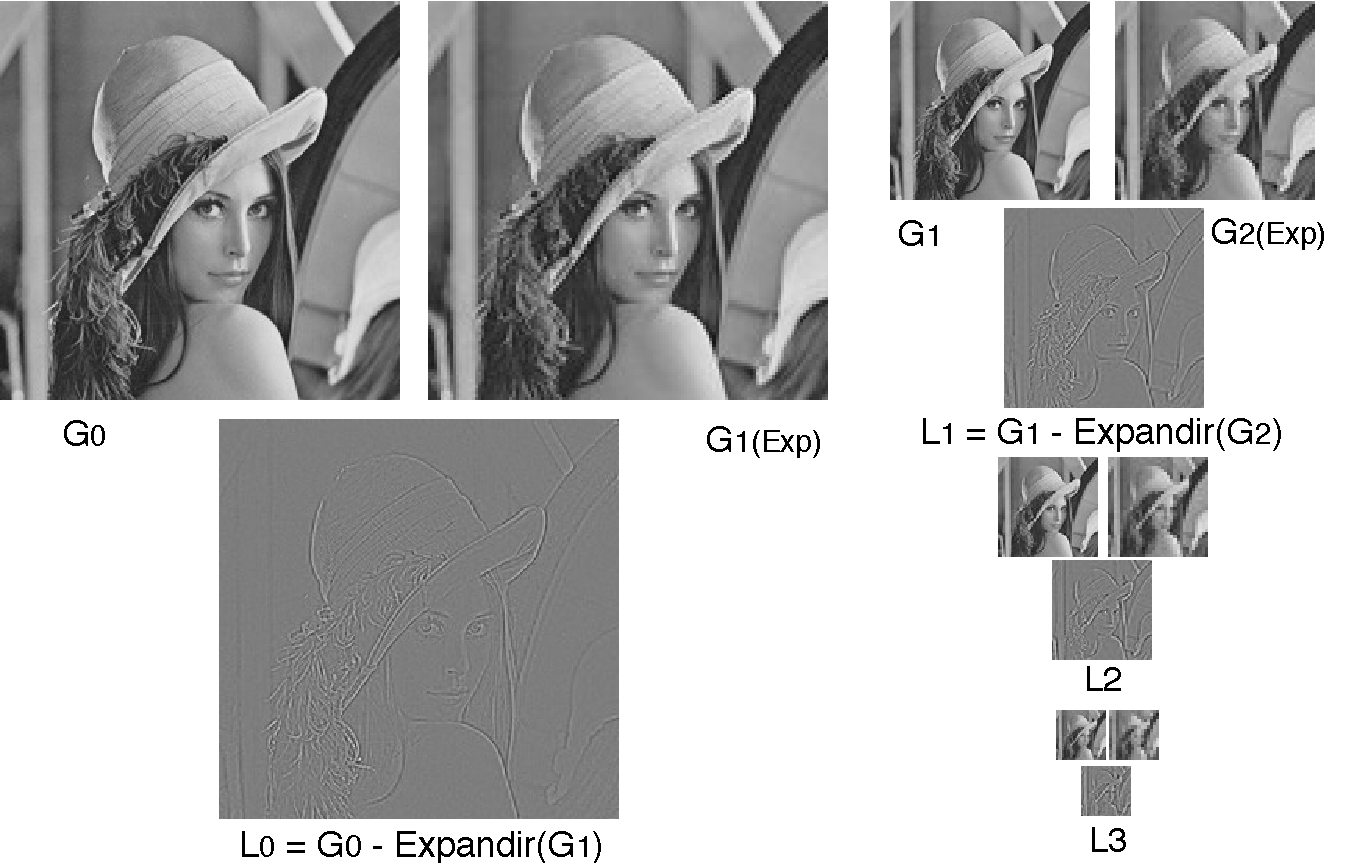
\includegraphics[width=.8\linewidth]{piramidal2.pdf}
	\caption[Construcción de pirámide de laplacianas]{Construcción de pirámide de laplacianas}
	\label{imagen:piramidal2}
\end{figure}

Una vez se tiene la pirámide de gaussianas, se elabora una pirámide de laplacianas utilizando \textit{DoG}, es decir, cada nivel de esta pirámide se construye restando un nivel de la pirámide gaussiana con su nivel siguiente pero expandido (para lograr las mismas dimensiones). Al restar una imagen con ella misma pero aplicada un filtro gaussiano --- que remueve las componentes en bajas frecuencias ---, se logra una imagen que resalte las componentes en las frecuencias altas. Esta composición se puede observar en la figura \ref{imagen:piramidal2}, donde a cada imagen laplaciana $L_i$ se le sumó una constante para efectos de visualización, ya que presenta valores muy bajos al aplicar únicamente la resta.

Como ya se mencionó, este proceso se aplica para imágenes que no comparten un área de superposición, con lo cual es necesario definir mediante una mascara binaria los límites de cada imagen. Convenientemente, el proceso de determinar la línea de corte ya nos ofrece esta máscara mediante el proceso de etiquetado, con lo cual se utiliza para definir las fronteras en esta fusión.

La pirámide gaussiana que se elaboró en un principio para cada imagen a fusionar, debe también crearse para la máscara, ya que la fusión debe realizarse en cada nivel de la pirámide. Finalmente para mostrar la imagen final en la resolución original, el proceso de fusión debe realizarse escalando cada nivel hasta las dimensiones originales.

Éste proceso consiste en expandir el último nivel de la pirámide --- con su respectiva mascara---, una vez expandido se le suma el laplaciano correspondiente, devolviéndole la componente en alta frecuencia que le fue removida. En este punto se tiene el par de imágenes expandidas un nivel, además de la mascara aun afectada por el efecto del filtro gaussiano, con lo cual se efectúa una suma ponderada entre las dos imágenes similar que en la sección \ref{feathering}, pero en este caso se utiliza la mascara difuminada para determinar el peso de la suma, y donde el inverso de la mascara determina la ponderación de la segunda imagen.

En la figura \ref{imagen:blend-apple} se puede observar el resultado de aplicar una fusión bajo el esquema piramidal.

\begin{figure}[H]
	\centering     %%% not \center
	\subfigure[]{\label{fig:apple}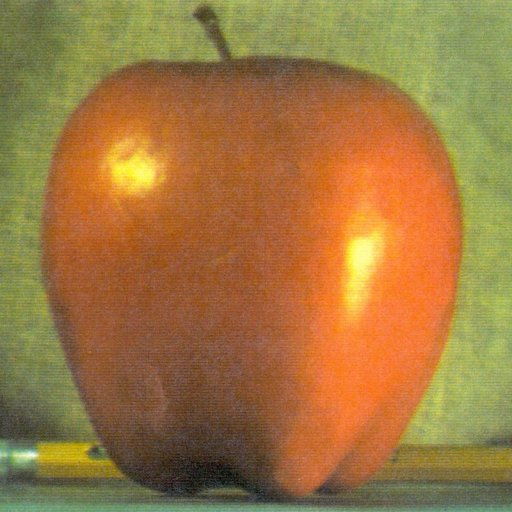
\includegraphics[width=.30\textwidth]{apple.jpg}}
	\subfigure[]{\label{fig:orange}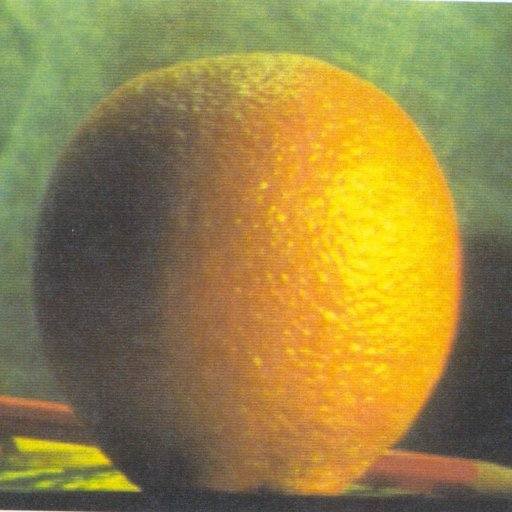
\includegraphics[width=.30\textwidth]{orange.jpg}}
	
	\subfigure[]{\label{fig:orange-mask}
\includegraphics[width=.30\textwidth]{mask.pdf}}
	\subfigure[]{\label{fig:apple-orange}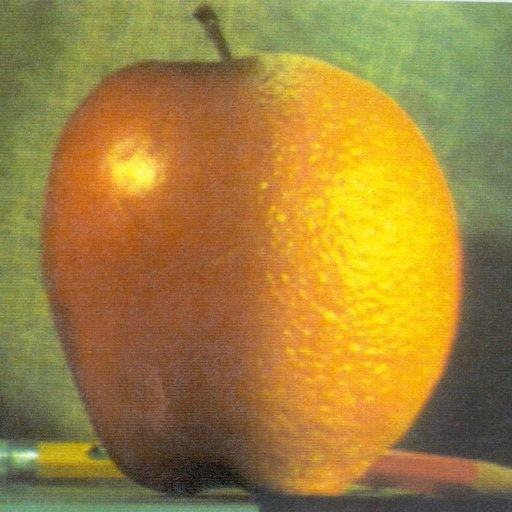
\includegraphics[width=.30\textwidth]{apple-orange.jpg}}
	
	\caption[Ejemplo de fusión pirámidal]{Fusión piramidal. Donde (a) y (b) representan las imágenes que se desean unir, (c) es la máscara para la fusión y (d) es el resultado final utilizando 9 bandas\protect\footnotemark.}
	\label{imagen:blend-apple}
\end{figure}
\footnotetext{ \url{https://compvisionlab.wordpress.com/2013/05/13/image-blending-using-pyramid/}}
%%%%%%%%%%%%%%%%%%%%%%%%%%%%%%%%%%%%%%%%%%%%%%%%%%%%%%%%%%%%%%%%%%%%%%%%%%%%%%%
\section{Resultados}

En esta sección se presentan los resultados de los algoritmos descritos en este capítulo, los cuales buscan reducir las discontinuidades y el error fotométrico en el mosaico final. Puesto que con este capítulo culmina la exposición de los módulos implementados, se presenta en la ultima parte resultados de los mosaicos obtenidos al emplear todo el sistema descrito. De esta forma se puede estudiar el rendimiento del sistema de generación de mosaico para distintos tipos de condiciones, y bajo distintas combinaciones de algoritmos.

\subsection*{Linea de corte}

A continuación se presentan los resultados del algoritmo descrito en la sección \ref{seccion-corte}.

En primer lugar estudiamos el caso en el que se tienen objetos en movimiento en el transcurso de la captura de imágenes. En la figura \ref{fig:corte:0233-a} se observa un par de imágenes alineadas según el esquema simple, en el cual se muestra completamente la ultima imagen añadida y ésta determina el borde entre las imágenes. Por otro lado en la figura \ref{fig:corte:0233-d} se muestra el mismo par unidas por la linea de corte que minimiza la diferencia entre dichas imágenes. Se aprecia también en las figuras \ref{fig:corte:0233-b} y \ref{fig:corte:0233-c} el etiquetado de píxeles (mascara) y la linea de corte respectivamente.

\begin{figure}[H]
	\centering     %%% not \center
	\subfigure[]{\label{fig:corte:0233-a}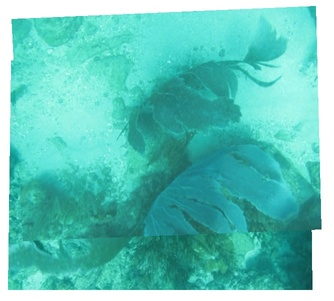
\includegraphics[width=.45\textwidth]{resultados/cut/0233-simple.jpg}}\hspace{0.005\textwidth}%
	\subfigure[]{\label{fig:corte:0233-b}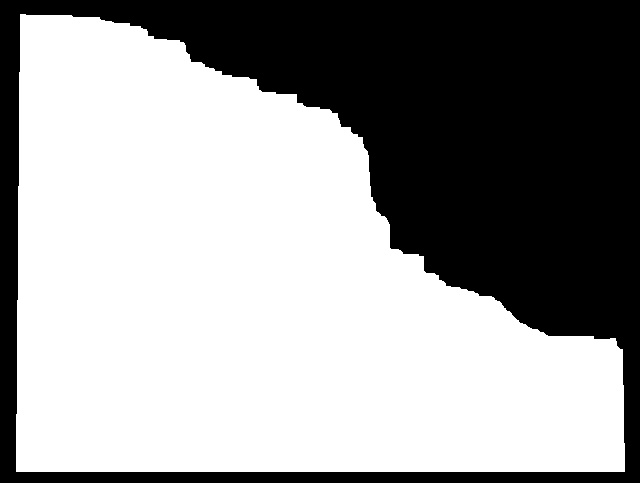
\includegraphics[width=.45\textwidth]{resultados/cut/0233-mask.jpg}}
	
	\subfigure[]{\label{fig:corte:0233-c}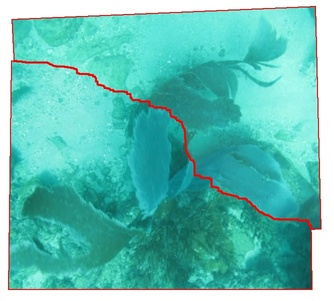
\includegraphics[width=.45\textwidth]{resultados/cut/0233-redline.jpg}}
	\subfigure[]{\label{fig:corte:0233-d}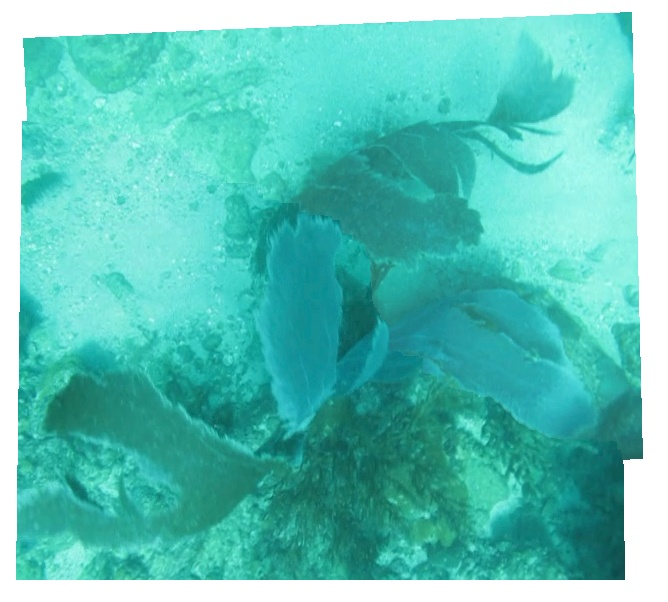
\includegraphics[width=.45\textwidth]{resultados/cut/0233-cutline.jpg}}

	\caption[Ejemplo de fusión pirámidal]{}
	\label{imagen:cut:0233}
\end{figure}

Una mejora importante que presenta este algoritmo, es que logra reducir y hasta eliminar el error producido por el efecto paralaje. En la figura \ref{fig:corte:0234-a} se observa un par de imágenes con un error de alineación producto de un objeto a distinta altura. Por otro lado en la figura \ref{fig:corte:0233-d} se puede ver como la mejor linea de corte logra eliminar el error anterior.

\begin{figure}[H]
	\centering     %%% not \center
	\subfigure[]{\label{fig:corte:0234-a}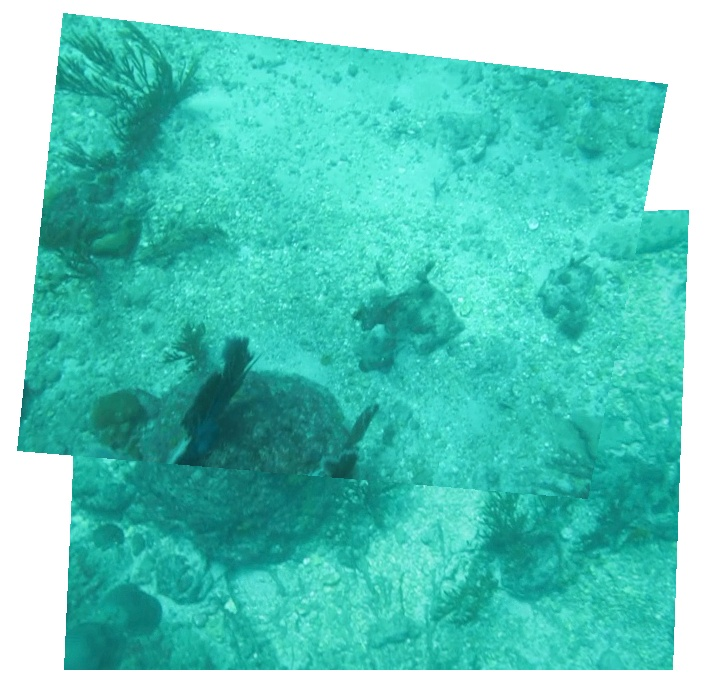
\includegraphics[width=.49\textwidth]{resultados/cut/0234-simple.jpg}}\hspace{0.05\textwidth}%
	\subfigure[]{\label{fig:corte:0234-b}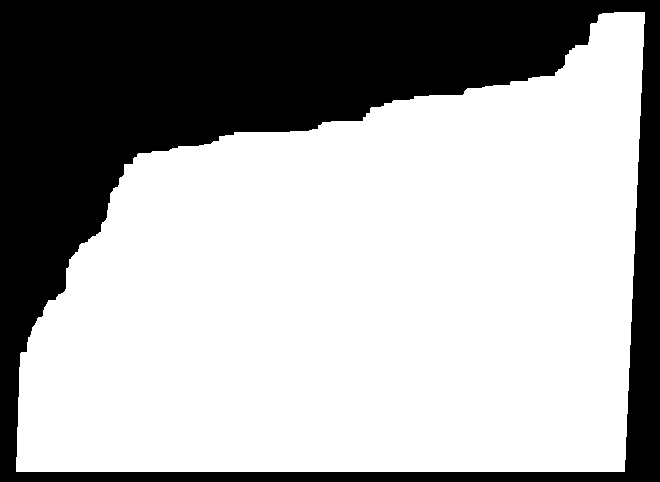
\includegraphics[width=.44\textwidth]{resultados/cut/0234-mask.jpg}}
	
	\subfigure[]{\label{fig:corte:0234-c}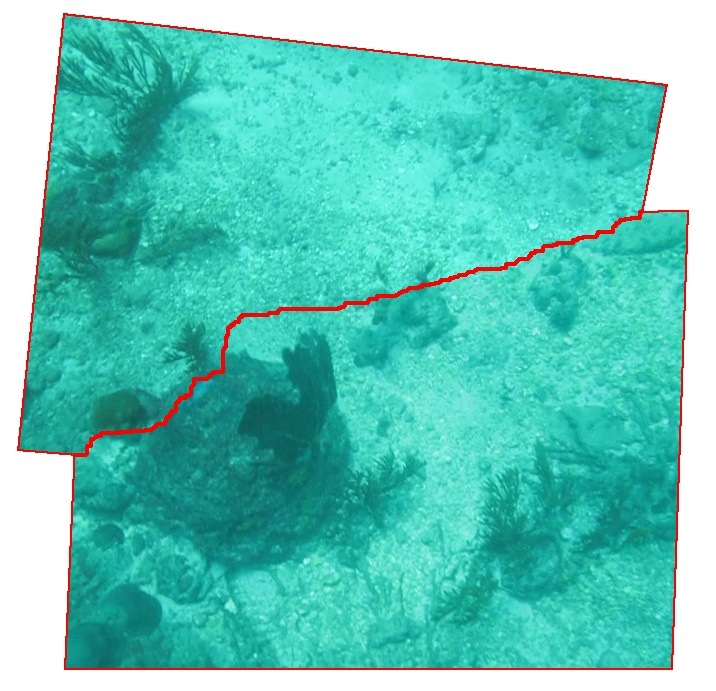
\includegraphics[width=.49\textwidth]{resultados/cut/0234-redline.jpg}}
	\subfigure[]{\label{fig:corte:0234-d}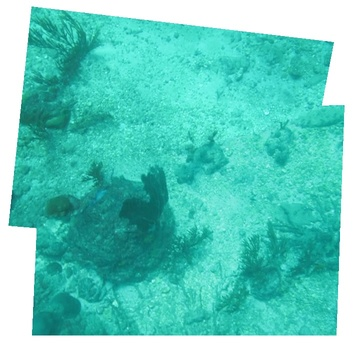
\includegraphics[width=.49\textwidth]{resultados/cut/0234-cutline.jpg}}
	
	\caption[Ejemplo de fusión pirámidal]{}
	\label{imagen:cut:0234}
\end{figure}

Ya hemos comentado sobre los posibles errores de alineación cuando se cuenta con distintos planos en una misma imagen. En la figura \ref{fig:corte:geo-a} se observa un par de imágenes que presentan un importante error de alineación sobre el plano en la parte inferior, mientras que en la parte superior, la sección elevada logra coincidir con el modelo hallado. En la figura \ref{fig:corte:geo-d} se aprecia el par de imágenes luego de unirse por la mejor linea de corte. Si bien se tiene un pequeño error en el costado izquierdo, se logra un par de imágenes sin discontinuidades entre ellas.

\begin{figure}[H]
	\centering     %%% not \center
	\subfigure[]{\label{fig:corte:geo-a}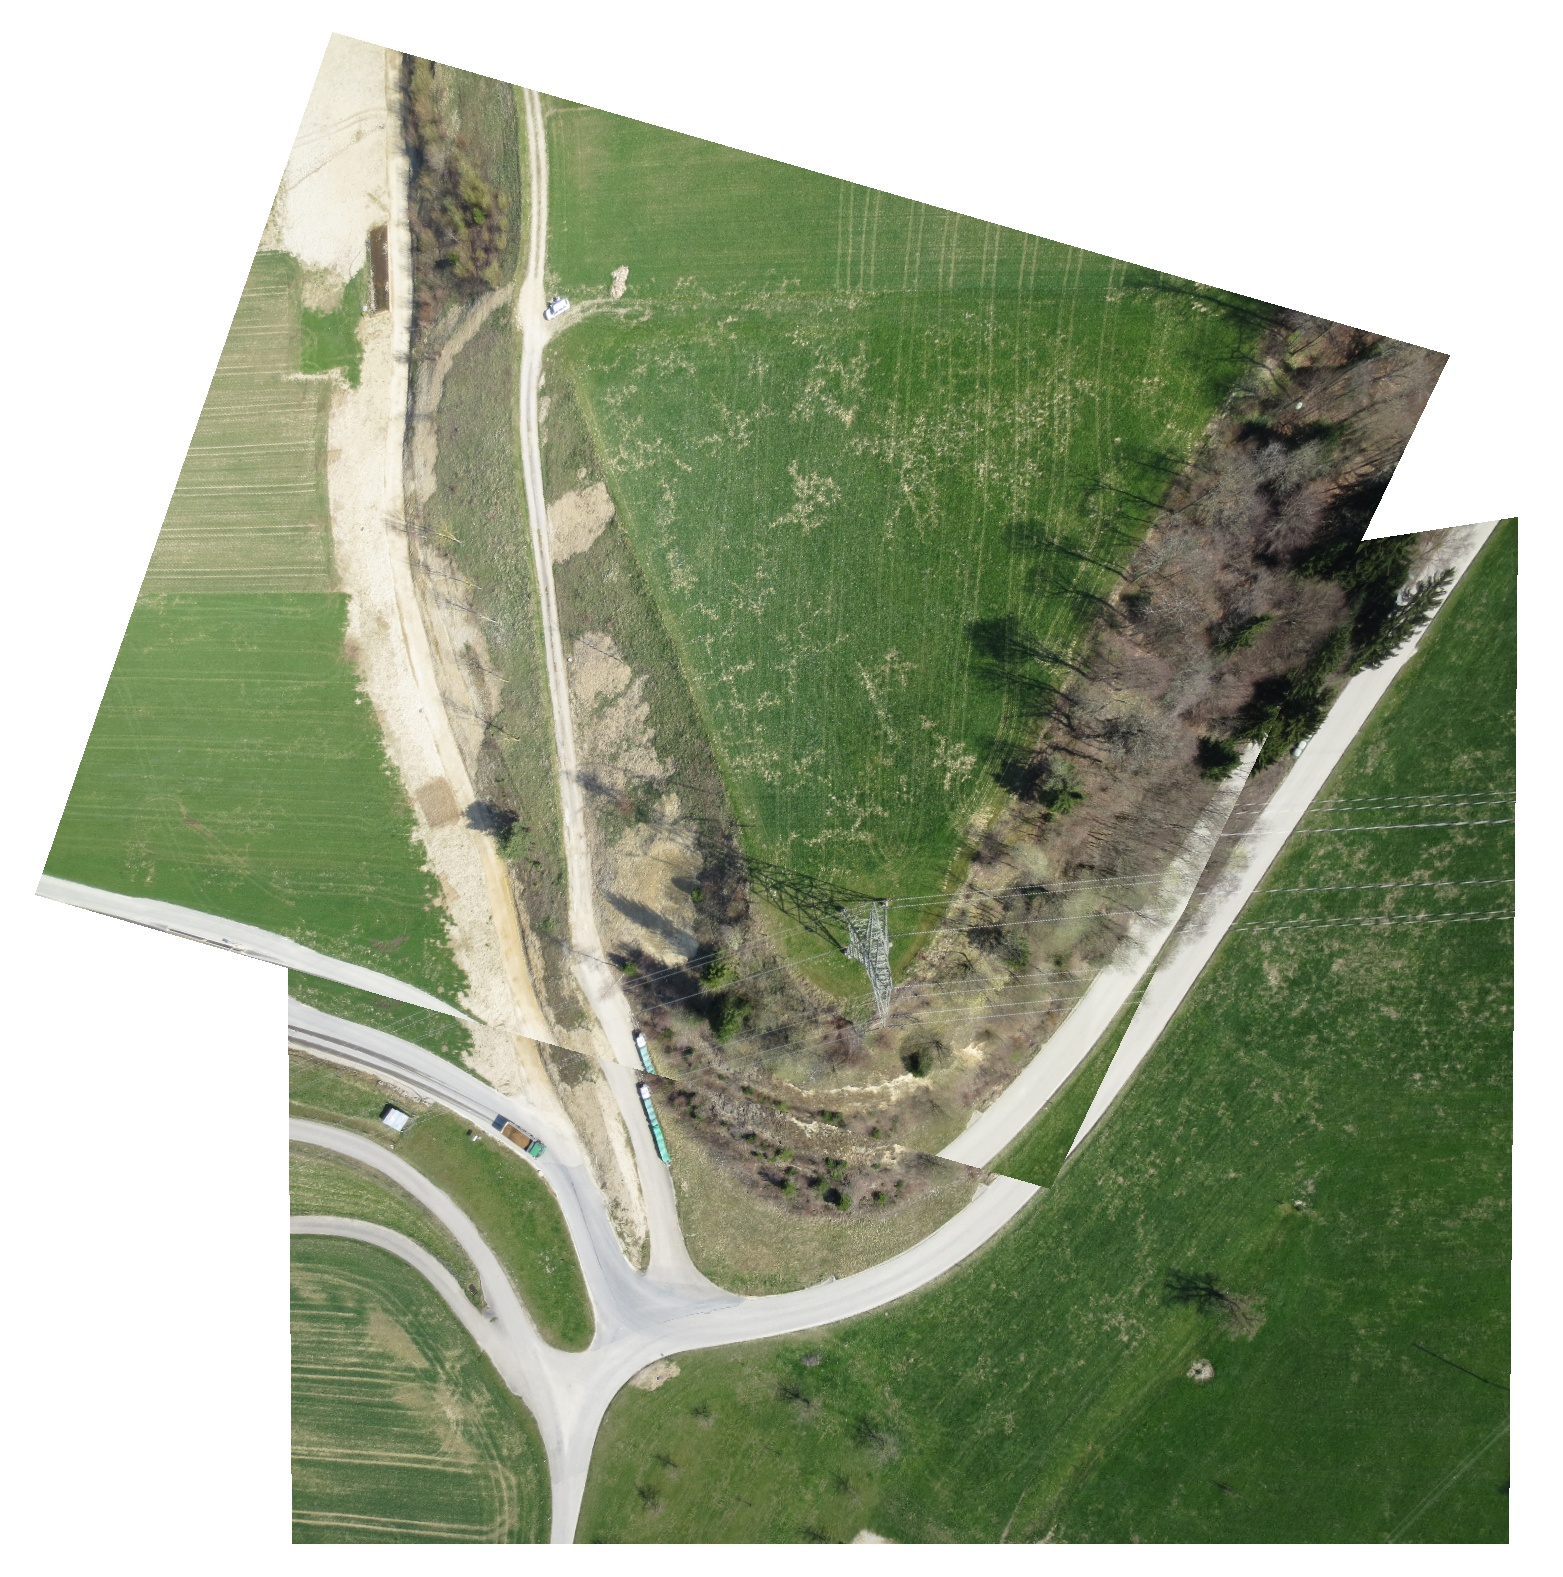
\includegraphics[width=.49\textwidth]{resultados/cut/geo-simple.jpg}}\hspace{0.1\textwidth}%
	\subfigure[]{\label{fig:corte:geo-b}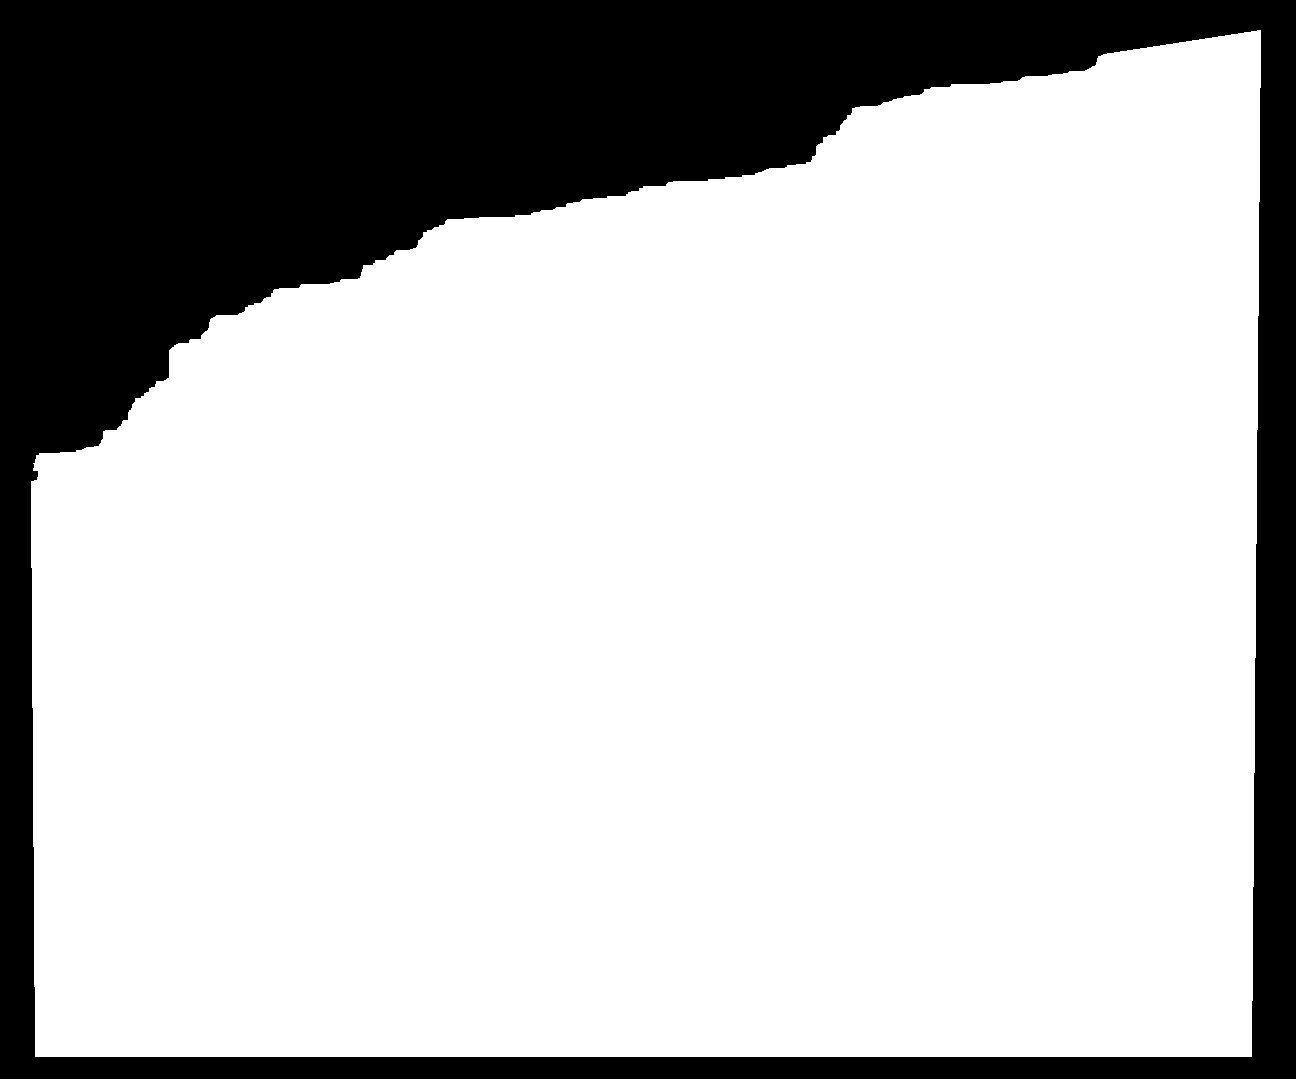
\includegraphics[width=.39\textwidth]{resultados/cut/geo-mask.jpg}}
	
	\subfigure[]{\label{fig:corte:geo-c}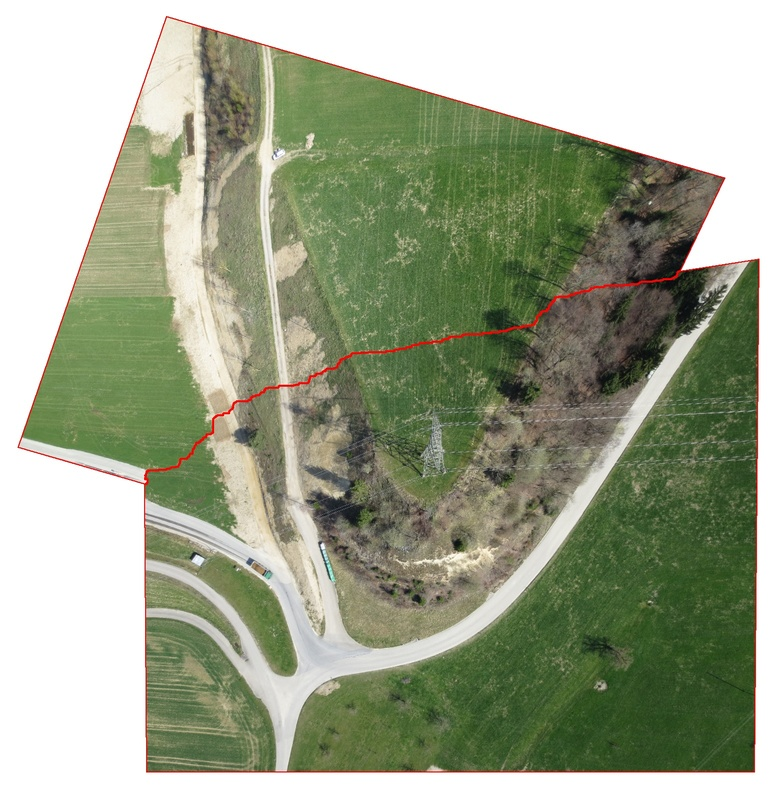
\includegraphics[width=.49\textwidth]{resultados/cut/geo-redline.jpg}}
	\subfigure[]{\label{fig:corte:geo-d}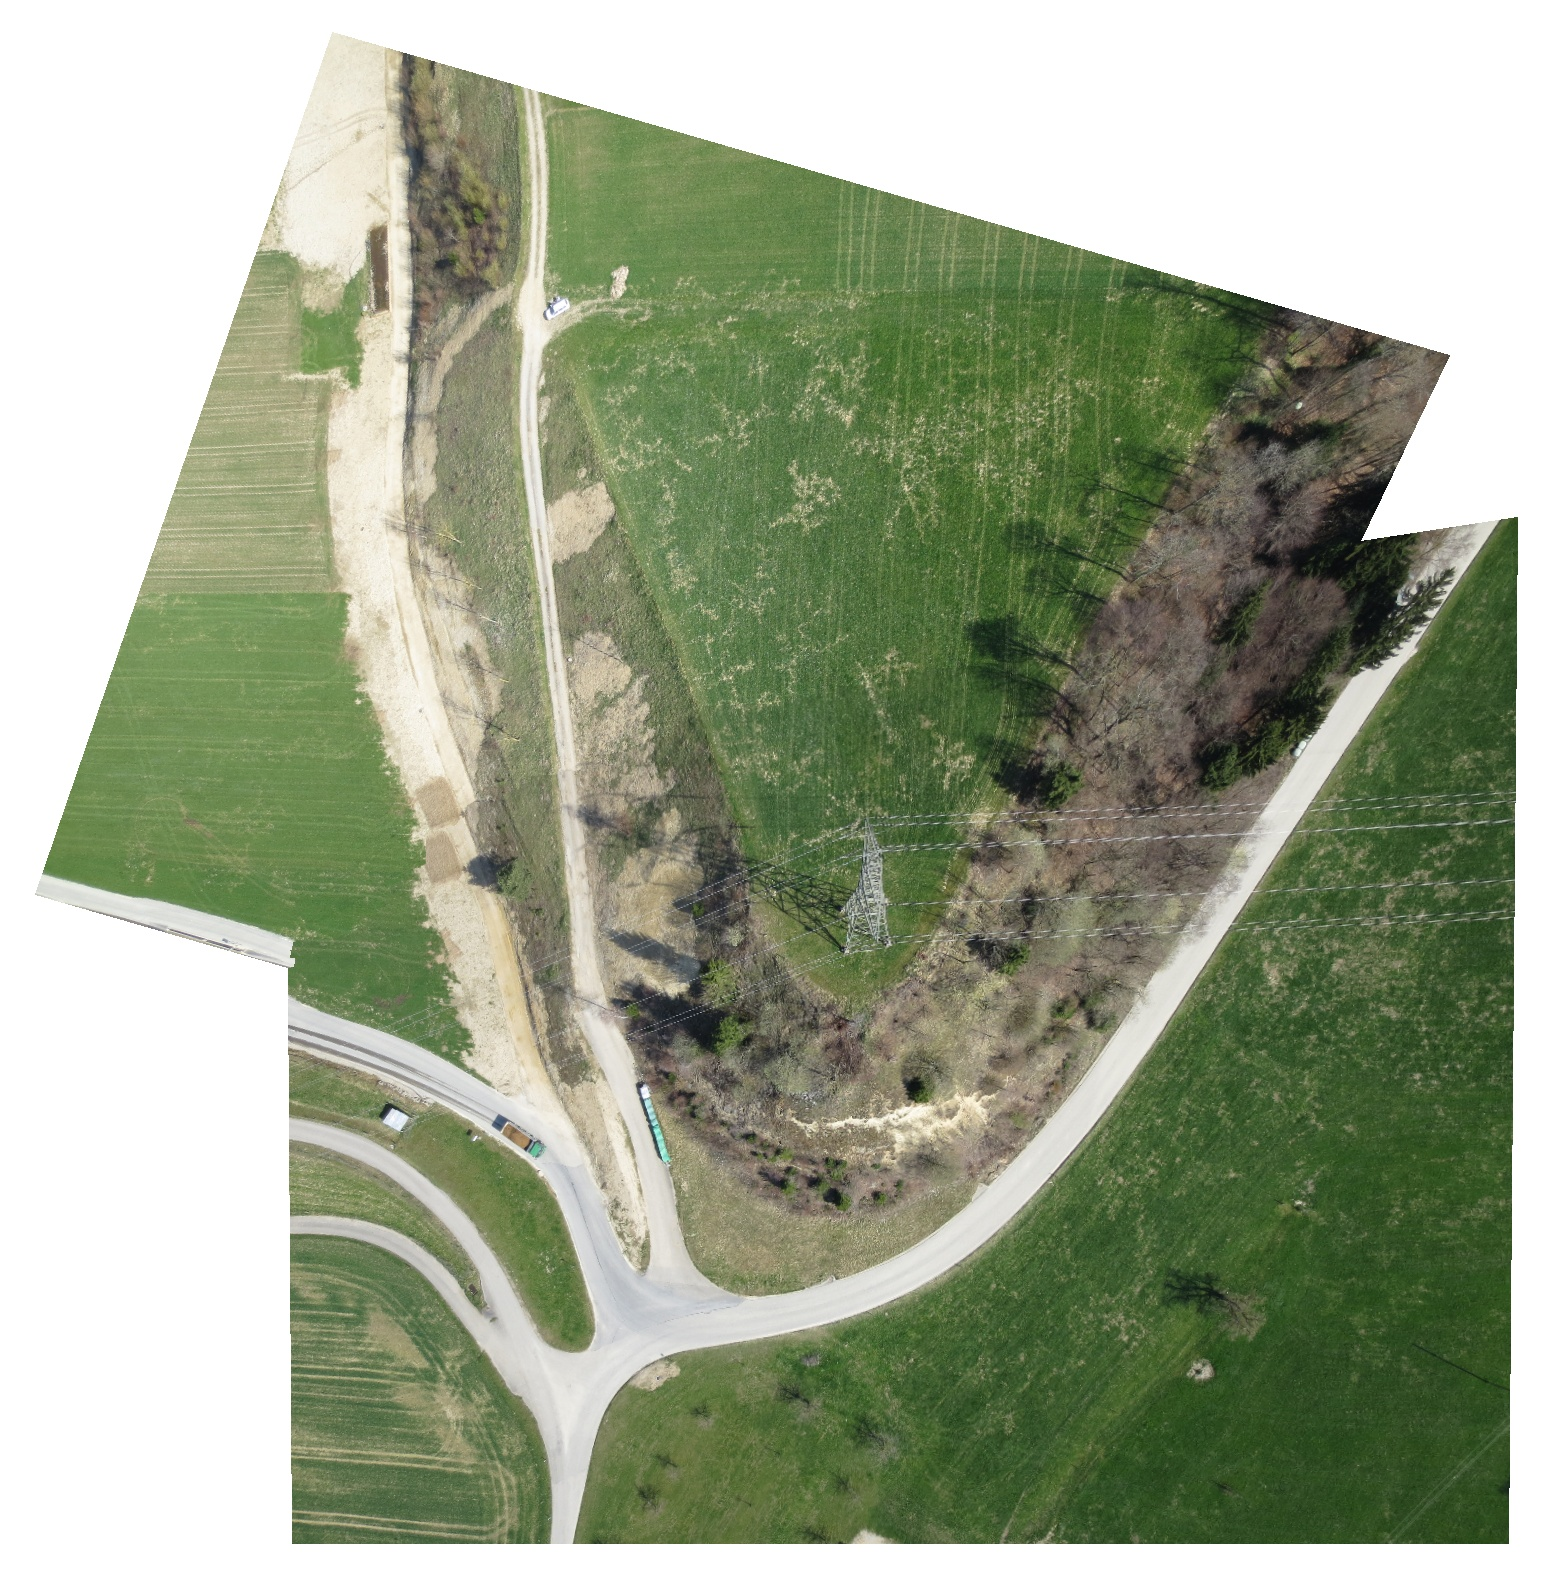
\includegraphics[width=.49\textwidth]{resultados/cut/geo-cutline.jpg}}
	
	\caption[Ejemplo de fusión pirámidal]{}
	\label{imagen:cut:geo}
\end{figure}

Hasta ahora se han presentado casos en los que se lidia con un par de imágenes. En esta oportunidad de tiene un mosaico compuesto por tres imágenes, en las cuales se tiene un error producto del efecto paralaje. En este caso el algoritmo busca por la mejor linea de corte para cada par de imágenes por separado, pero logrando un mosaico final sin errores de discontinuidades.

En este ejemplo en particular se logra evidenciar una debilidad que tiene este algoritmo. Si bien es muy robusto bordeando objetos por la diferencia de texturas y bordes, es común que se cuente con discontinuidades visuales producto de cambios de iluminación.

\begin{figure}[ht]
	\centering     %%% not \center
	\subfigure[]{\label{fig:corte:espenky-a}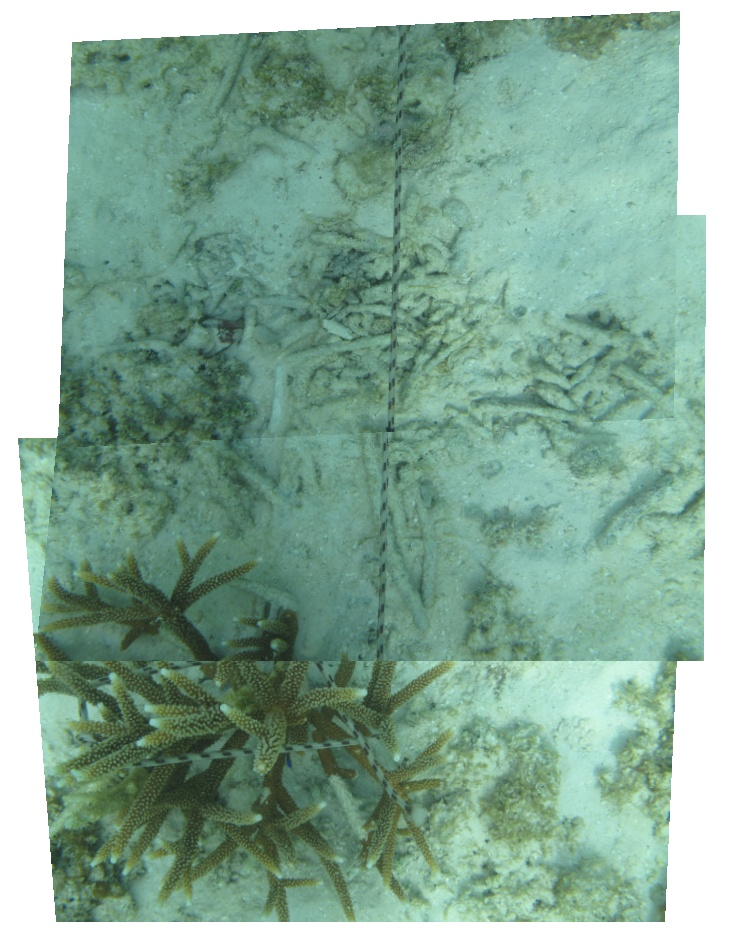
\includegraphics[width=.47\textwidth]{resultados/cut/Espenky-simple.jpg}}
	\subfigure[]{\label{fig:corte:espenky-b}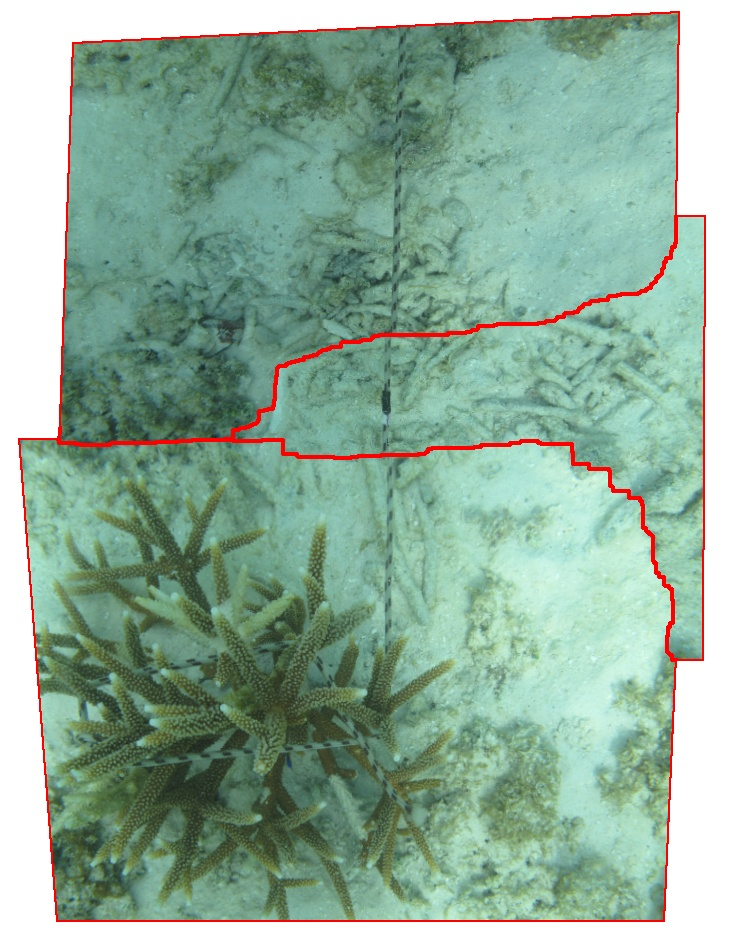
\includegraphics[width=.47\textwidth]{resultados/cut/Espenky-redline.jpg}}
	
	\subfigure[]{\label{fig:corte:espenky-c}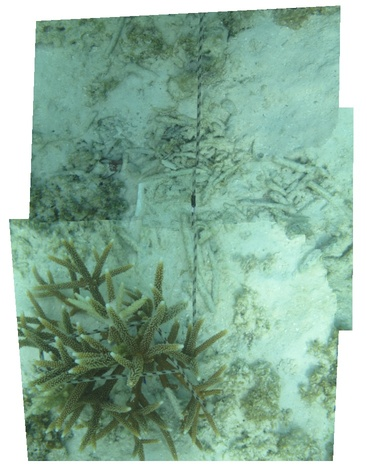
\includegraphics[width=.47\textwidth]{resultados/cut/Espenky-cutline.jpg}}
	
	\caption[Ejemplo de fusión pirámidal]{}
	\label{imagen:cut:espenky}
\end{figure}


\subsection*{Corrección de color}

A continuación se presentan los resultados de aplicar el algoritmo en la sección \ref{seccion-color}.

De los resultados del algoritmo que busca la mejor linea de corte, se tiene que es susceptible a errores de discontinuidad producto de cambios en la exposición de luz entre imágenes, con lo cual es necesario equilibrar tal diferencia para lograr mejor continuidad en el mosaico final.

En la figura \ref{fig:color:geo-a} se observa un mosaico compuesto por tres imágenes, donde una de ellas presenta un cambio importante en la intensidad de luz. Aplicando el método descrito es posible reducir este error, tal y como se muestra en la figura \ref{fig:color:geo-b}.

\begin{figure}[H]
	\centering     %%% not \center
	\subfigure[]{\label{fig:color:geo-a}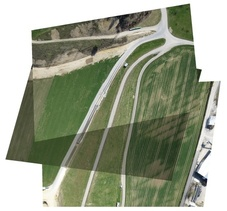
\includegraphics[width=.49\textwidth]{resultados/color/geo-no.jpg}}
	\subfigure[]{\label{fig:color:geo-b}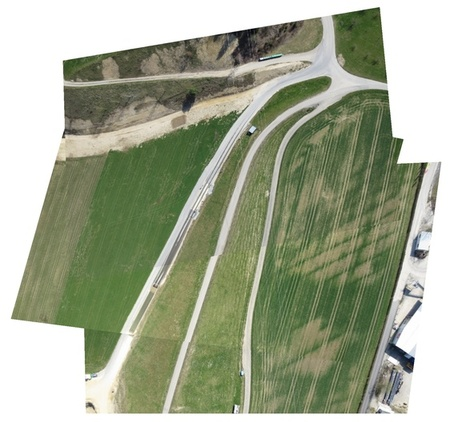
\includegraphics[width=.49\textwidth]{resultados/color/geo-si.jpg}}
	
	\caption[Ejemplo de fusión pirámidal]{}
	\label{imagen:color:geo}
\end{figure}

Del ejemplo anterior se tiene que la imagen irregular presenta poca iluminación con respecto al resto. Caso distinto se tiene para el siguiente conjunto presentado en la figura \ref{imagen:color:0233}, donde se muestra en \ref{fig:color:geo-a} y \ref{fig:color:geo-b} el mosaico sin y con corrección de color respectivamente. 

\begin{figure}[H]
	\centering     %%% not \center
	\subfigure[]{\label{fig:color:0233-a}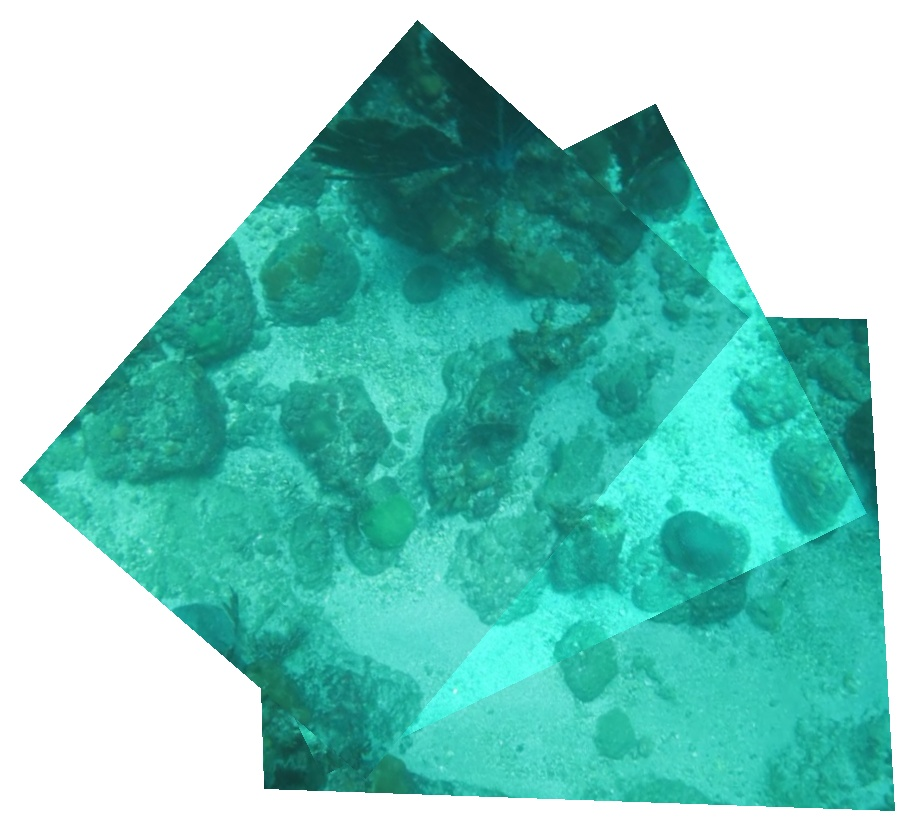
\includegraphics[width=0.49\textwidth]{resultados/color/0233-no.jpg}}
	\subfigure[]{\label{fig:color:0233-b}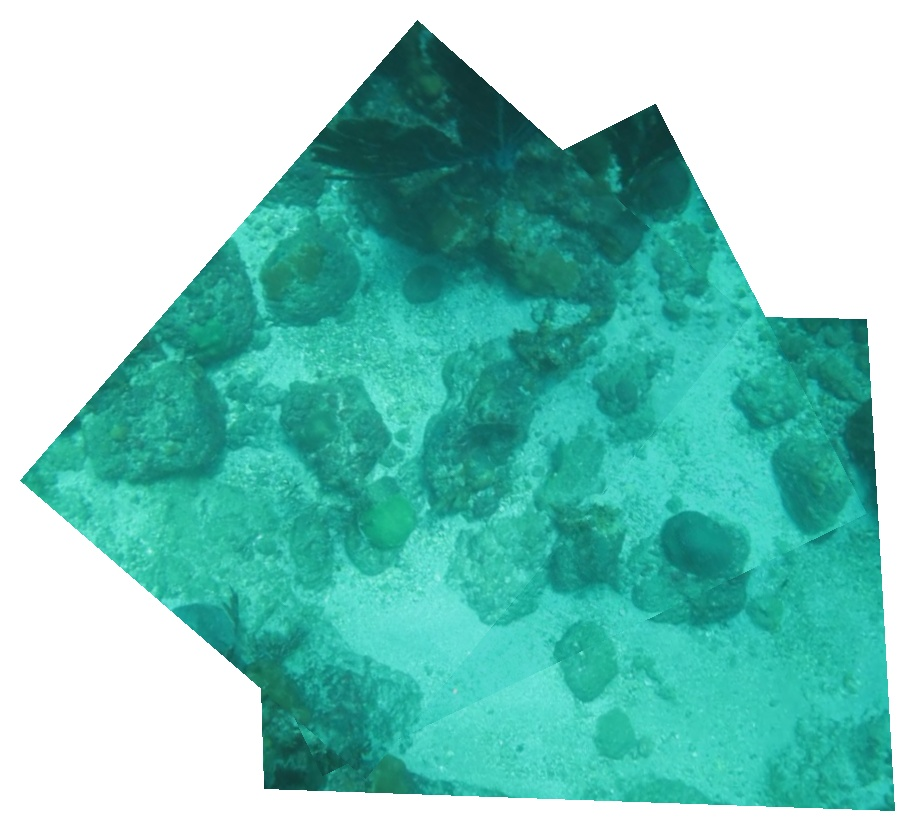
\includegraphics[width=0.49\textwidth]{resultados/color/0233-si.jpg}}
	
	\caption[Ejemplo de fusión pirámidal]{}
	\label{imagen:color:0233}
\end{figure}

Para los mosaicos anteriores se estudiaron casos en los que se tenia un cambio de iluminación uniformemente distribuido a lo largo de toda la imagen, con lo cual el se lograba un resultado deseado al utilizar un método de corrección de color lineal.

A continuación se presenta el caso en los que este cambio se produce en secciones de una imagen. En la figura \ref{fig:color:espenky-a} se observa un mosaico que presenta diversas variaciones de iluminación, tanto entre imágenes como también entre secciones de algunas de estas. Luego de aplicar la corrección de color se logra el mosaico de la figura \ref{fig:color:espenky-b}, donde si bien se observa una mejora global en la intensidad de iluminación, se tienen regiones en las cuales esta diferencia se acentúa.

\begin{figure}[H]
	\centering     %%% not \center
	\subfigure[]{\label{fig:color:espenky-a}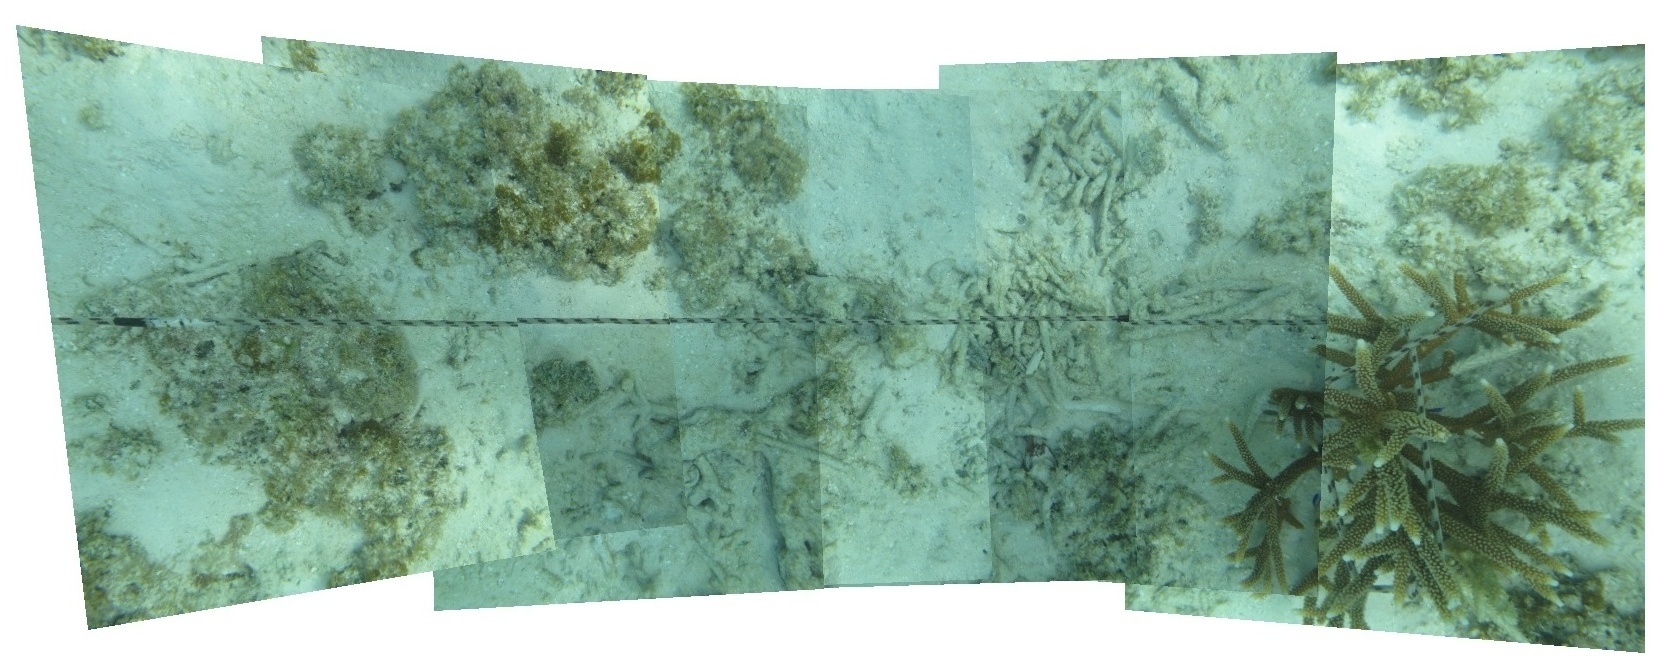
\includegraphics[width=0.8\textwidth]{resultados/color/espenky-no.jpg}}
	\subfigure[]{\label{fig:color:espenky-b}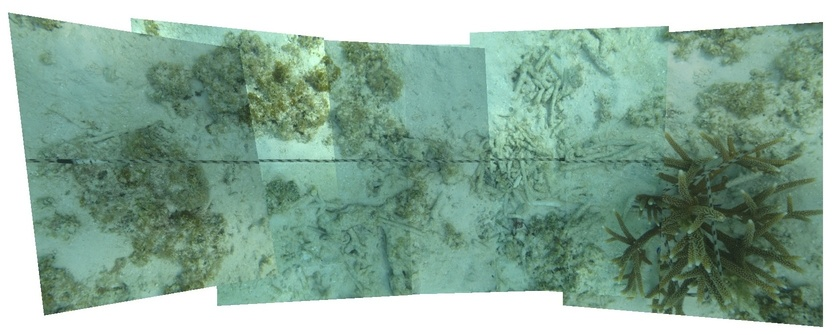
\includegraphics[width=0.8\textwidth]{resultados/color/espenky-si.jpg}}
	
	\caption[Ejemplo de fusión pirámidal]{}
	\label{imagen:color:espenky}
\end{figure}

\subsection*{Fusión ponderada}

A continuación se presentan los resultados del algoritmo descrito en la sección \ref{seccion-fusion}.

Ya se ha observado como los algoritmos presentados anteriormente logran solventar la mayoría de inconvenientes y errores de alineación en las imágenes. Pero también se observó como se presentan casos ante los cuales los resultados no corresponden con los deseados. El siguiente ejemplo ilustra un conjunto de imágenes estudiadas anteriormente, y como se logra resolver a través de este algoritmo los errores de discontinuidad que no pudieron ser corregidos en pasos anteriores. En la figura \ref{imagen:blend:espenky} se observa como se logra reducir la discontinuidad producida por un cambio de iluminación, aplicando la fusión piramidal para distintos niveles de escalas.

\begin{figure}[h]
	\centering
	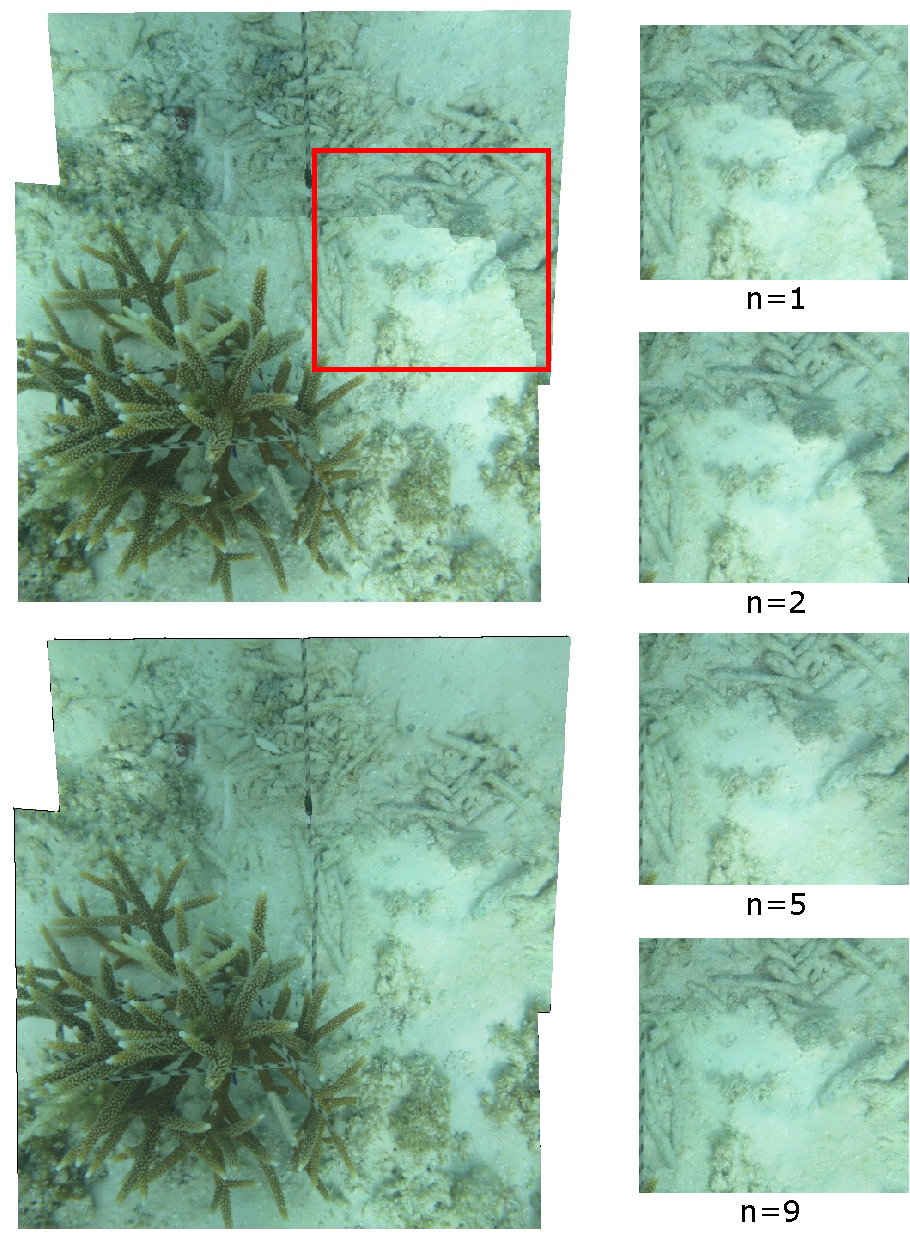
\includegraphics[width=0.75\linewidth]{/resultados/blend/blend-espenky3.pdf}
	\caption[Fusión pirámidal]{Fusión pirámidal}
	\label{imagen:blend:espenky}
\end{figure}

Es posible evaluar la calidad de la fusión de las imágenes utilizando la derivada de la imagen final, con la cual es posible identificar bordes debido a cambios o discontinuidades entre estas. En la figura \ref{imagen:blend:laplacian} podemos identificar el cambio producido en la derivada de la imagen luego de aplicar el algoritmo de fusión, donde podemos observar en la figura \ref{fig:blend:laplacian-b} como el borde es difuminado completamente, logrando una transición suavizada y una línea de corte indetectable en la imagen final. 

\begin{figure}[H]
	\centering     %%% not \center
	\subfigure[]{\label{fig:blend:laplacian-a}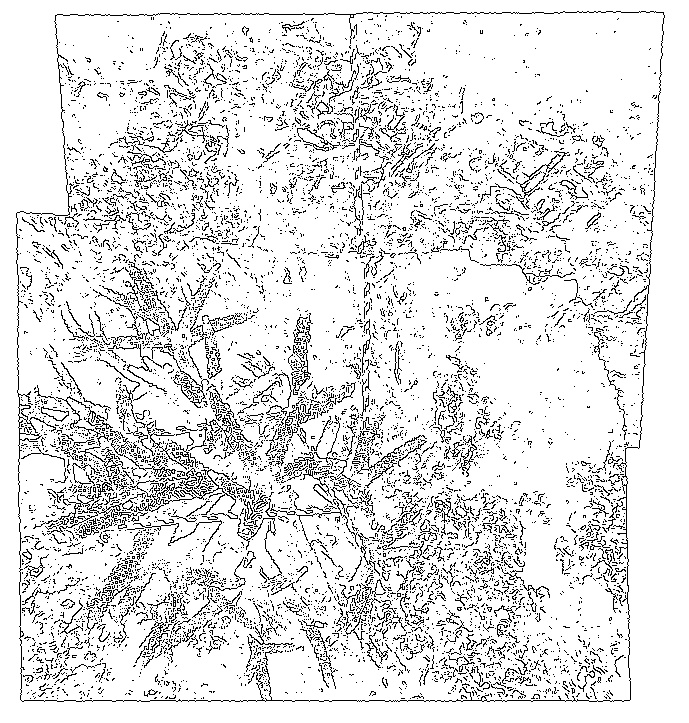
\includegraphics[width=0.49\textwidth]{resultados/blend/canny00.jpg}}
	\subfigure[]{\label{fig:blend:laplacian-b}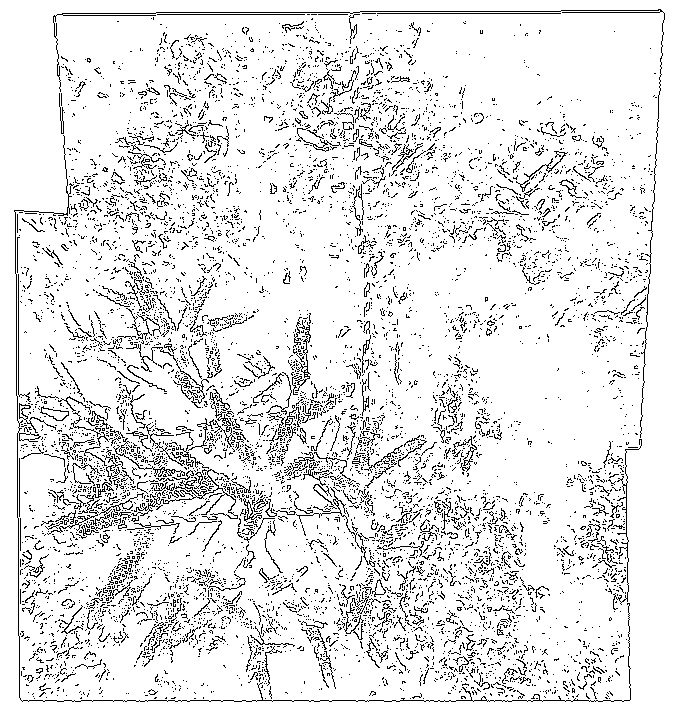
\includegraphics[width=0.49\textwidth]{resultados/blend/canny09.jpg}}
	
	\caption[Fusión pirámidal]{}
	\label{imagen:blend:laplacian}
\end{figure}

\subsection*{Mosaicos completos}

\begin{figure}[h]
	\centering     %%% not \center
	\subfigure[]{\label{fig:apple}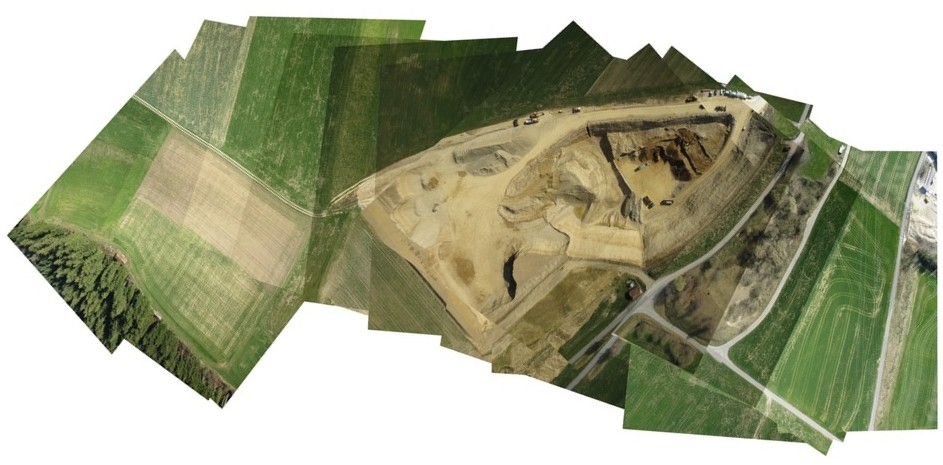
\includegraphics[width=0.9\textwidth]{resultados/full/geo2-0.jpg}}
	\subfigure[]{\label{fig:orange}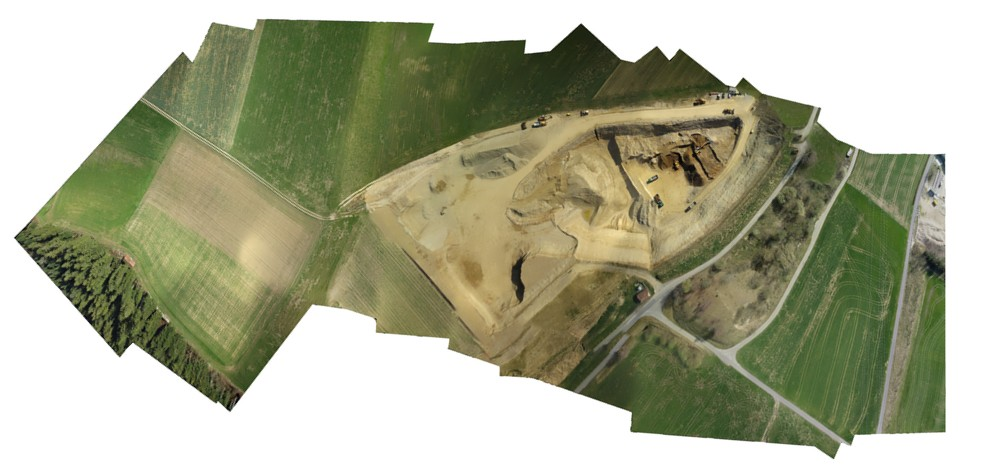
\includegraphics[width=0.9\textwidth]{resultados/full/geo2-1.jpg}}
	\subfigure[]{\label{fig:orange}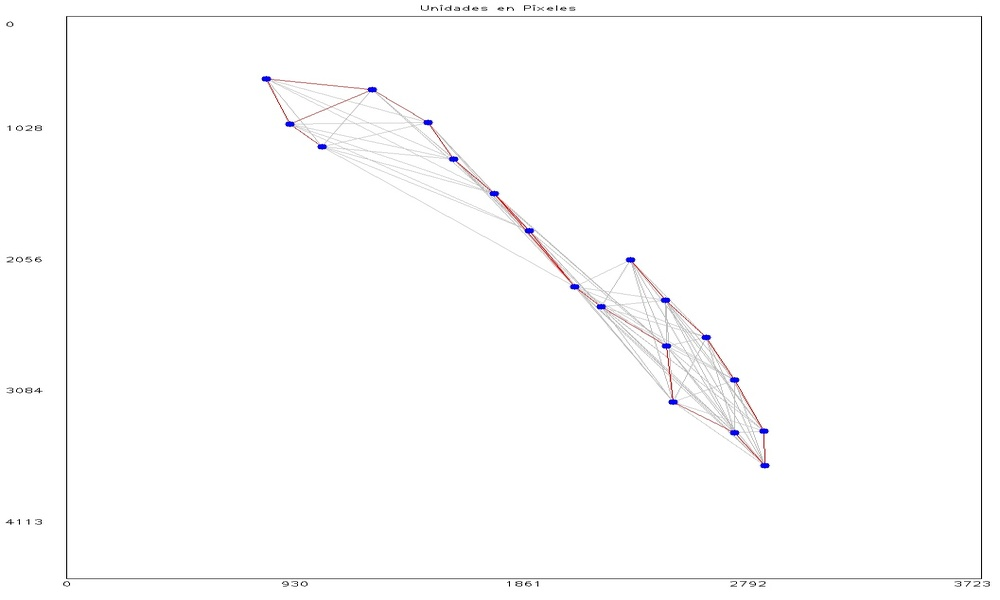
\includegraphics[width=0.8\textwidth]{resultados/full/geo2-map.jpg}}
		
	\caption[Fusión pirámidal]{}
	\label{imagen:full:geo2}
\end{figure}

\begin{figure}[h]
	\centering     %%% not \center
	\subfigure[]{\label{fig:apple}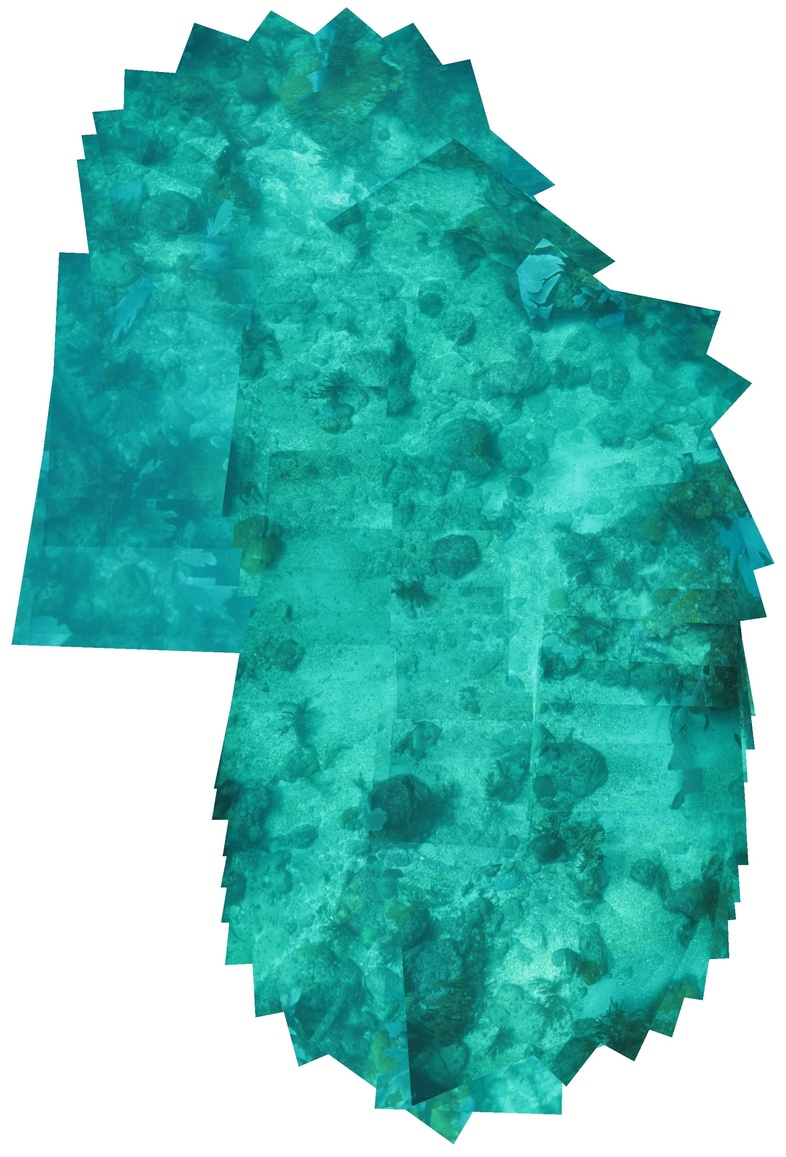
\includegraphics[width=0.9\textwidth]{resultados/full/0234-0.jpg}}
	\subfigure[]{\label{fig:orange}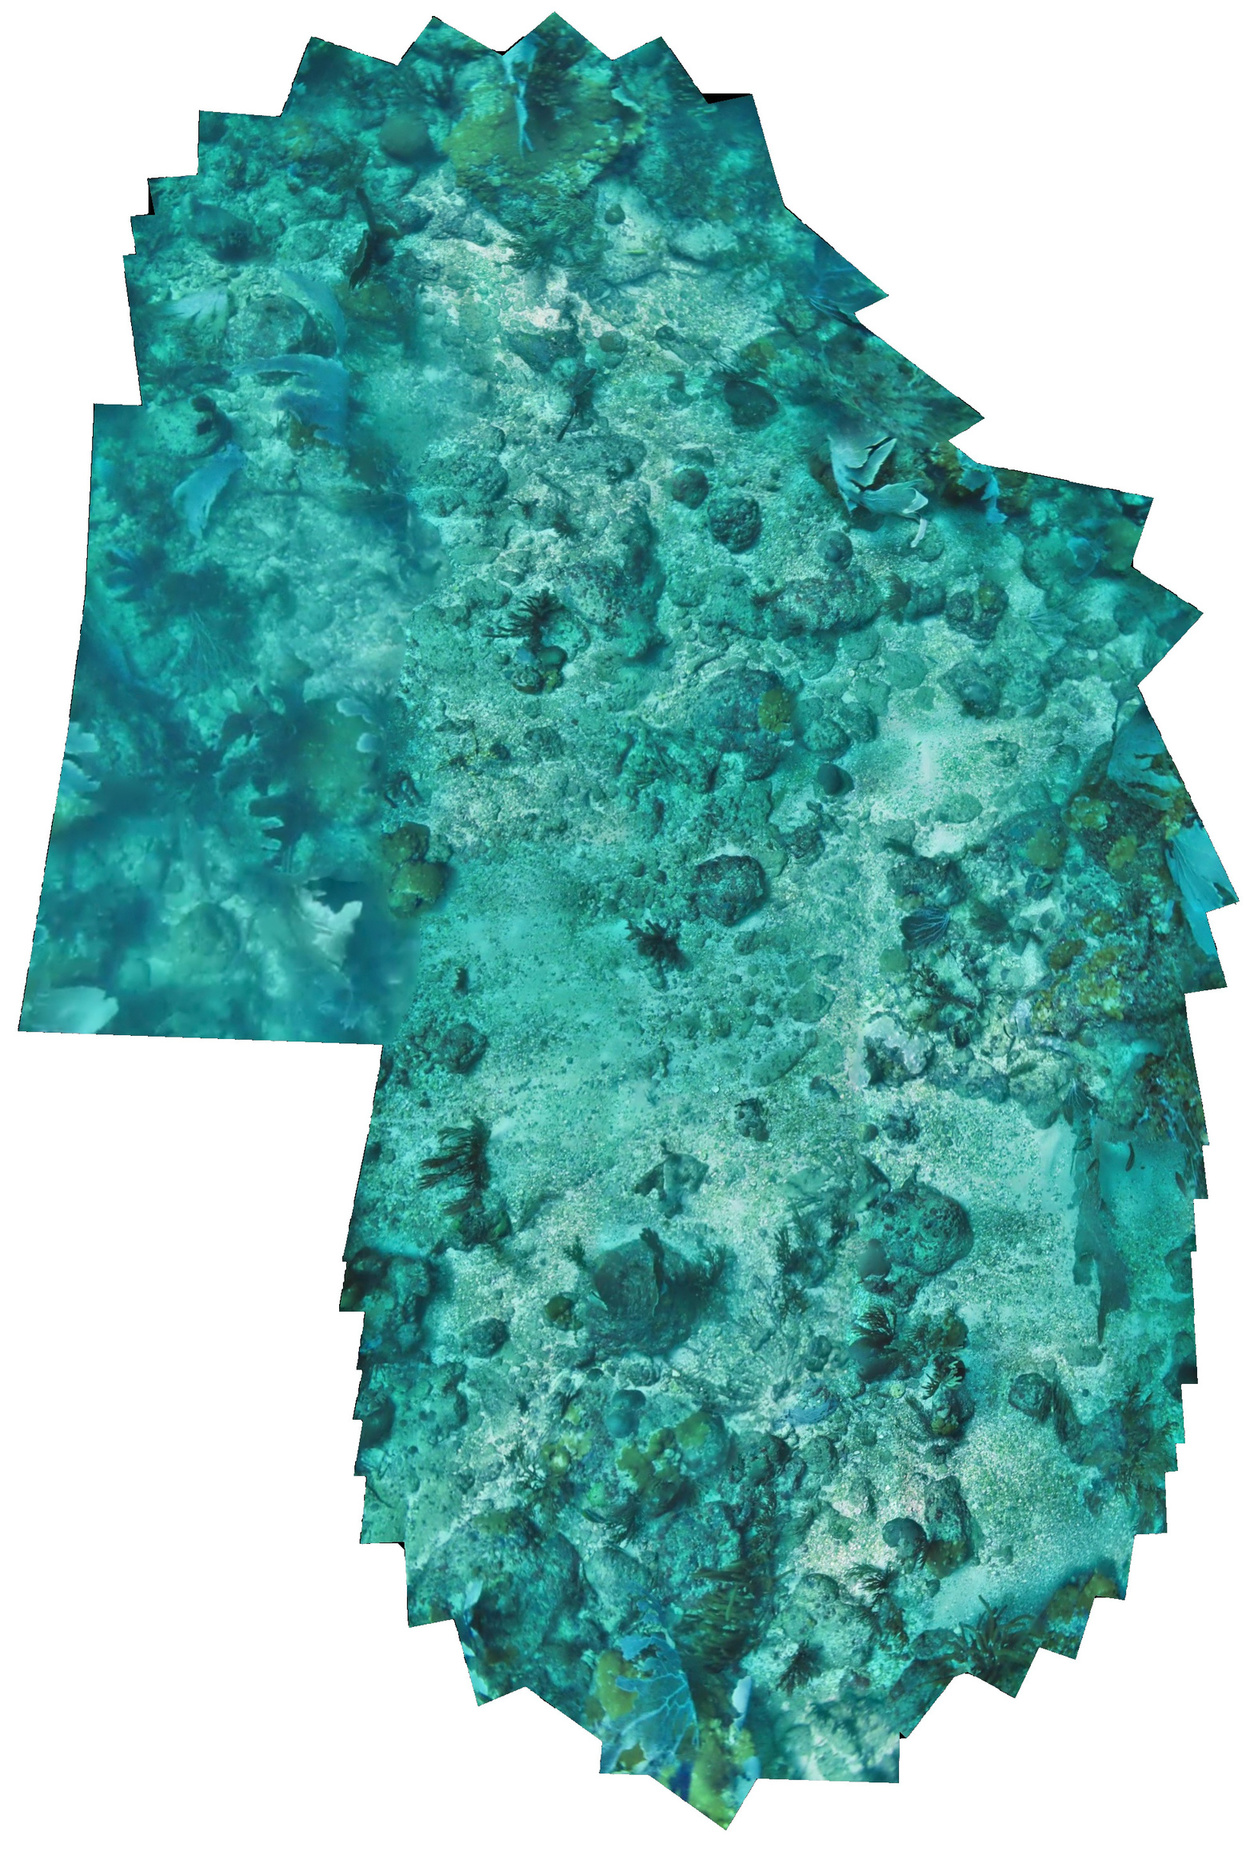
\includegraphics[width=0.9\textwidth]{resultados/full/0234-1.jpg}}
	\subfigure[]{\label{fig:orange}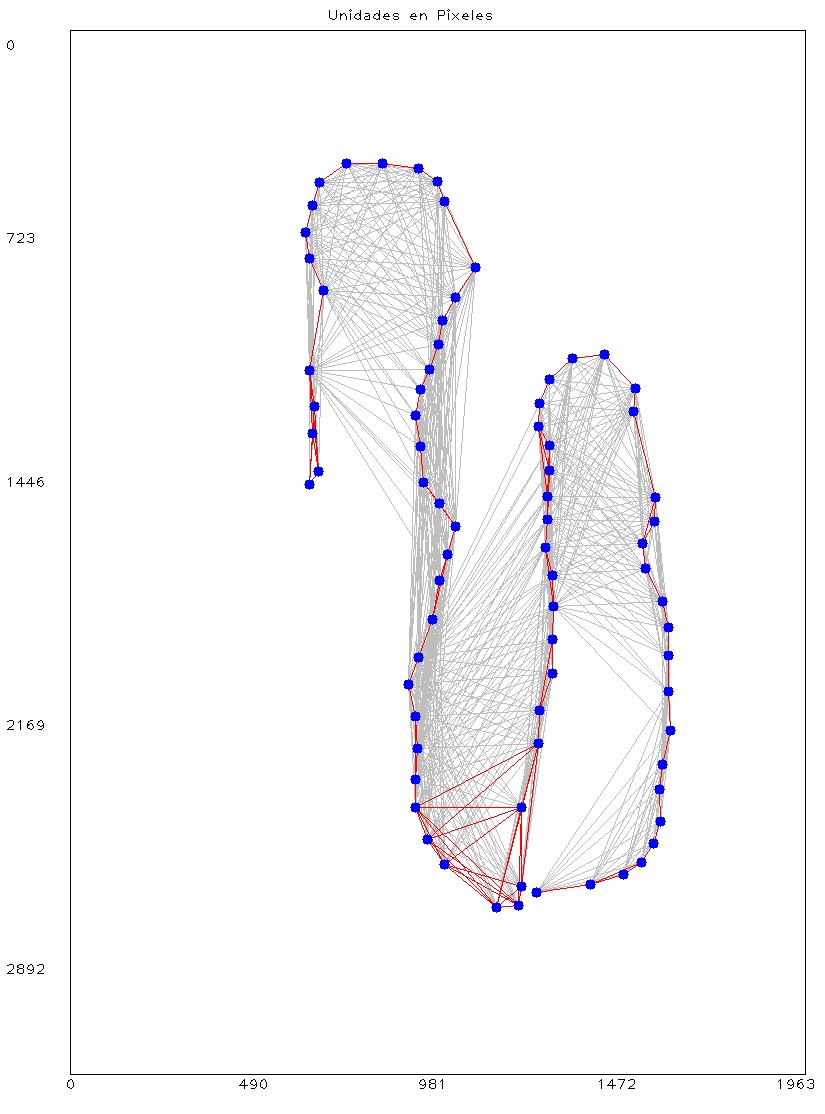
\includegraphics[width=0.8\textwidth]{resultados/full/0234-map.jpg}}
	
	\caption[Fusión pirámidal]{}
	\label{imagen:full:0234}
\end{figure}

\section{Resumen}
test
